% Se pre-carga la información del estudiante sólo para poder emplear el macro de
% selección de versión (digital o impresa)
% ===============================================================================
% El estudiante debe llenar sus datos en esta sección para que la plantilla los 
% auto-importe y genere automáticamente las páginas de portada y de firmas 
% autorizadas.
% ===============================================================================
% Datos del estudiante:
% -------------------------------------------------------------------------------
% Nombre completo
\def \nombreestudiante {Erick Stiv Junior Guerra Muñoz}
% Carné
\def \uvgcarne {21781}
% Facultad
\def \uvgfacultad {Ingeniería}
% Carrera
\def \uvgcarrera {Ingeniería en Ciencias de la Computación y Tecnologías de la Información}

% Datos del trabajo:
% -------------------------------------------------------------------------------
% Título completo
\def \titulotesis {Ciudadano Digital: La Inteligencia Artifcial como herramienta de acompañamiento informal en educación sobre ciudadanía y valores morales.}
% Año de entrega
\def \anoentrega {2025}
% Asesor
\def \nombreasesor {MA. Luis Furlán}

% Datos del tribunal examinador:
% -------------------------------------------------------------------------------
% Nombre del primer examinador
\def \nombreprimerex {MSc. Douglas Barrios}
% Nombre del segundo examinador
\def \nombresegundoex {PhD. Gabriel Barrientos}
% Año de aprobación
\def \anoaprobacion {2025}

% Capítulos pre-definidos
% -------------------------------------------------------------------------------
% Comentar las líneas de las secciones que desean omitirse, por defecto se 
% se incluyen todas.


% Formato y estilo de la plantilla
% -------------------------------------------------------------------------------
% Modo impresión: Puede des-comentar la siguiente línea para generar un documento pdf sin la portada, para cuando se desee imprimir el documento para encuadernación
%\def \printver {Versión del documento para impresión}

% Portada: Puede cambiarse la imagen en la portada al cambiar el nombre del 
% archivo siguiente. NOTA: debe tener la suficiente resolución para cubrir el área
% designada
\def \imagenportada {plantilla/portadacit.jpg}

% Referencias: Puede des-comentar la siguiente línea para utilizar el formato de referencias APA
%\def \usarAPA {Usar formato APA}

% Párrafo: Puede comentar la siguiente línea si desea emplear un formato de 
% párrafo distinto al establecido por defecto
\def \parpordefecto {Formato de párrafo por defecto}

% Capítulos y secciones: Puede des-comentar la siguiente línea para establecer el
% formato de los capítulos y secciones bajo el estándar original de UVG para
% trabajos de graduación. Este incluye: capítulos con numeración romana, secciones
% con letras mayúsculas, sub-secciones con números y sub-sub-secciones con letras
% minúsculas
%\def \capsecuvg {Formato UVG para capítulos y secciones}

\ifdefined\printver
    \documentclass[11pt, letterpaper, twoside, openright]{report}
\else
    \documentclass[11pt, letterpaper]{report}
\fi

% Eliminar la opción de twoside y openright si se desea generar la versión
% digital del documento en lugar de la versión impresa
%\documentclass[11pt, letterpaper, twoside, openright]{report}
\usepackage[spanish, es-nodecimaldot, es-noquoting]{babel}
% cambiar a spanish, mexico si se quiere emplear tabla en lugar de cuadro
\selectlanguage{spanish}
\usepackage[utf8]{inputenc}
\usepackage[T1]{fontenc}

\title{Plantilla para Trabajos de Graduación IE-MT 2019v3}
\author{MSc. Miguel Zea}
\date{\today}

% Información del estudiante en el archivo datos_estudiante.tex
% ===============================================================================
% El estudiante debe llenar sus datos en esta sección para que la plantilla los 
% auto-importe y genere automáticamente las páginas de portada y de firmas 
% autorizadas.
% ===============================================================================
% Datos del estudiante:
% -------------------------------------------------------------------------------
% Nombre completo
\def \nombreestudiante {Erick Stiv Junior Guerra Muñoz}
% Carné
\def \uvgcarne {21781}
% Facultad
\def \uvgfacultad {Ingeniería}
% Carrera
\def \uvgcarrera {Ingeniería en Ciencias de la Computación y Tecnologías de la Información}

% Datos del trabajo:
% -------------------------------------------------------------------------------
% Título completo
\def \titulotesis {Ciudadano Digital: La Inteligencia Artifcial como herramienta de acompañamiento informal en educación sobre ciudadanía y valores morales.}
% Año de entrega
\def \anoentrega {2025}
% Asesor
\def \nombreasesor {MA. Luis Furlán}

% Datos del tribunal examinador:
% -------------------------------------------------------------------------------
% Nombre del primer examinador
\def \nombreprimerex {MSc. Douglas Barrios}
% Nombre del segundo examinador
\def \nombresegundoex {PhD. Gabriel Barrientos}
% Año de aprobación
\def \anoaprobacion {2025}

% Capítulos pre-definidos
% -------------------------------------------------------------------------------
% Comentar las líneas de las secciones que desean omitirse, por defecto se 
% se incluyen todas.


% Formato y estilo de la plantilla
% -------------------------------------------------------------------------------
% Modo impresión: Puede des-comentar la siguiente línea para generar un documento pdf sin la portada, para cuando se desee imprimir el documento para encuadernación
%\def \printver {Versión del documento para impresión}

% Portada: Puede cambiarse la imagen en la portada al cambiar el nombre del 
% archivo siguiente. NOTA: debe tener la suficiente resolución para cubrir el área
% designada
\def \imagenportada {plantilla/portadacit.jpg}

% Referencias: Puede des-comentar la siguiente línea para utilizar el formato de referencias APA
%\def \usarAPA {Usar formato APA}

% Párrafo: Puede comentar la siguiente línea si desea emplear un formato de 
% párrafo distinto al establecido por defecto
\def \parpordefecto {Formato de párrafo por defecto}

% Capítulos y secciones: Puede des-comentar la siguiente línea para establecer el
% formato de los capítulos y secciones bajo el estándar original de UVG para
% trabajos de graduación. Este incluye: capítulos con numeración romana, secciones
% con letras mayúsculas, sub-secciones con números y sub-sub-secciones con letras
% minúsculas
%\def \capsecuvg {Formato UVG para capítulos y secciones}
% ================================================================================
% En este archivo se colocan opciones adicionales para modificar el formato de la
% plantilla, para emplearse en otros tipos de documentos que no sean trabajos de
% graduación. Si usted está trabajando su tesis, NO modifique este archivo
% ================================================================================
% Capítulos pre-definidos
% --------------------------------------------------------------------------------
% Comentar las líneas de las secciones que desean omitirse, por defecto se 
% se incluyen todas.
\def \CAPportada {Portada}
\def \CAPcaratula {Caratula}
\def \CAPcaratula {Caratula}
\def \CAPfirmas {Hoja de firmas}

%Opcionales
% Dedicatoria / Reconocimiento (opcional)
% \def \CAPdedicatoria {Dedicatoria}
% \def \CAPprefacio {Prefacio}

\def \CAPresumen {Resumen}
% Abstract
\def \CAPabstract {Resumen}

%Tablas de contenido
\def \CAPindice {Índice general}
\def \CAPcuadros {Listado de tablas}
\def \CAPalgoritmos {Listado de algoritmos}
% \def \CAPfiguras {Listado de figuras}
% \def \CAPglosario {Glosario}

\def \CAPintroduccion {Introducción}

%Opcionales
\def \CAPjustificacion {Justificación}
% \def \CAPantecedentes {Antecedentes}

\def \CAPobjetivos {Objetivos}

%Opcionales
% \def \CAPalcance {Alcances}

\def \CAPmarcoteorico {Marco teórico}
% Metodología
\def \CAPmetodologia {Metodología}
% Resultados
\def \CAPresultados {Resultados}
% Discusión
\def \CAPdiscusion {Discusión}
\def \CAPconclusiones {Conclusiones}
%\def \CAPrecomendaciones {Recomendaciones}
\def \CAPbibliografia {Bibliografía}

% Opcionales
% \def \CAPanexos {Anexos}
% Apéndice
% \def \CAPapendice {Apéndice}

% ==============================================================================
% DEFINICIÓN DE PAQUETES
% ==============================================================================
\usepackage{xcolor}
\usepackage{amsfonts}
\usepackage{amsmath}
\usepackage{amssymb}
\usepackage{amsthm}
\usepackage{amsfonts}
\usepackage{mathtools}
\usepackage{graphicx}
\usepackage{xfrac}
\usepackage{float}
\usepackage{mathtools}
\usepackage[hypertexnames=false]{hyperref}
% \usepackage{bookmark}
\usepackage[font=small]{caption}
\usepackage{subcaption}
%\usepackage{csquotes}
\usepackage{xpatch}
\usepackage{emptypage}
\usepackage{hyphenat}
\usepackage{fancyhdr}
\ifdefined\usarAPA
  \usepackage[backend=biber, style=apa]{biblatex}
\else
  \usepackage[backend=biber, style=ieee, sorting=none, citestyle=numeric-comp]{biblatex}
\fi
\addbibresource{q-bibliografia.bib}

\usepackage[percent]{overpic}

\usepackage{chngcntr}

\ifdefined\CAPglosario
	%\usepackage[toc]{glossaries}
	\usepackage[numberedsection]{glossaries}
	\makeglossaries
    \newglossaryentry{latex}
{
    name=latex,
    description={Es un lenguaje de marcado adecuado especialmente para la creación de documentos científicos}
} 
 
\newglossaryentry{formula}
{
    name=fórmula,
    description={Una expresión matemática} 
}
\fi

% ==============================================================================
% MÁRGENES Y FORMATO GENERALES
% ==============================================================================
\usepackage[top=1in, left=1.5in, right=1in, bottom=1in]{geometry}
%Options: Sonny, Lenny, Glenn, Conny, Rejne, Bjarne, Bjornstrup
\usepackage[Sonny]{fncychap}

% ==============================================================================
% DEFINICIONES DE LA PLANTILLA
% ==============================================================================
\graphicspath{ {figuras/} }
\definecolor{uvg-green}{RGB}{17,71,52}
\newcommand{\defaultparformat}[1]{
	{\setlength{\parskip}{2ex}
     \input{#1}}
}
\ifdefined\capsecuvg
	\renewcommand\thechapter{\Roman{chapter}}
    \renewcommand\thesection{\Alph{section}}
	\renewcommand\thesubsection{\arabic{subsection}}
    \renewcommand\thesubsubsection{\alph{subsubection}}
\fi
\counterwithout{figure}{chapter}
\counterwithout{table}{chapter}
\counterwithout{equation}{chapter}

\newcommand{\blankpage}{
\newpage
\thispagestyle{empty}
\mbox{}
\newpage
}
% ==============================================================================

% Comandos definidos por el usuario en el archivo comandos_usuario.tex
\input{2-paquetes_y_comandos_usuario}

% ==============================================================================
% CUERPO DEL TRABAJO
% ==============================================================================
\pagestyle{headings}
\begin{document}

% ==============================================================================
% PORTADA
% ==============================================================================
\ifdefined\printver
    \let\CAPportada\undefined
\fi 

\ifdefined\CAPportada
    \cleardoublepage\phantomsection
    % \pdfbookmark{Portada}{toc}
	\newgeometry{left=3cm, bottom=0in, top=1in, right=3cm}
	\pagecolor{uvg-green}
	\thispagestyle{empty}

	\color{white}
	\noindent \hrulefill \par
	\vspace{0.1in}
	\noindent \Huge \nohyphens{\titulotesis} \par
	\noindent \hrulefill \par
	\noindent
	\LARGE \nombreestudiante

	\begin{figure}[b!]
    	%\makebox[\textwidth]{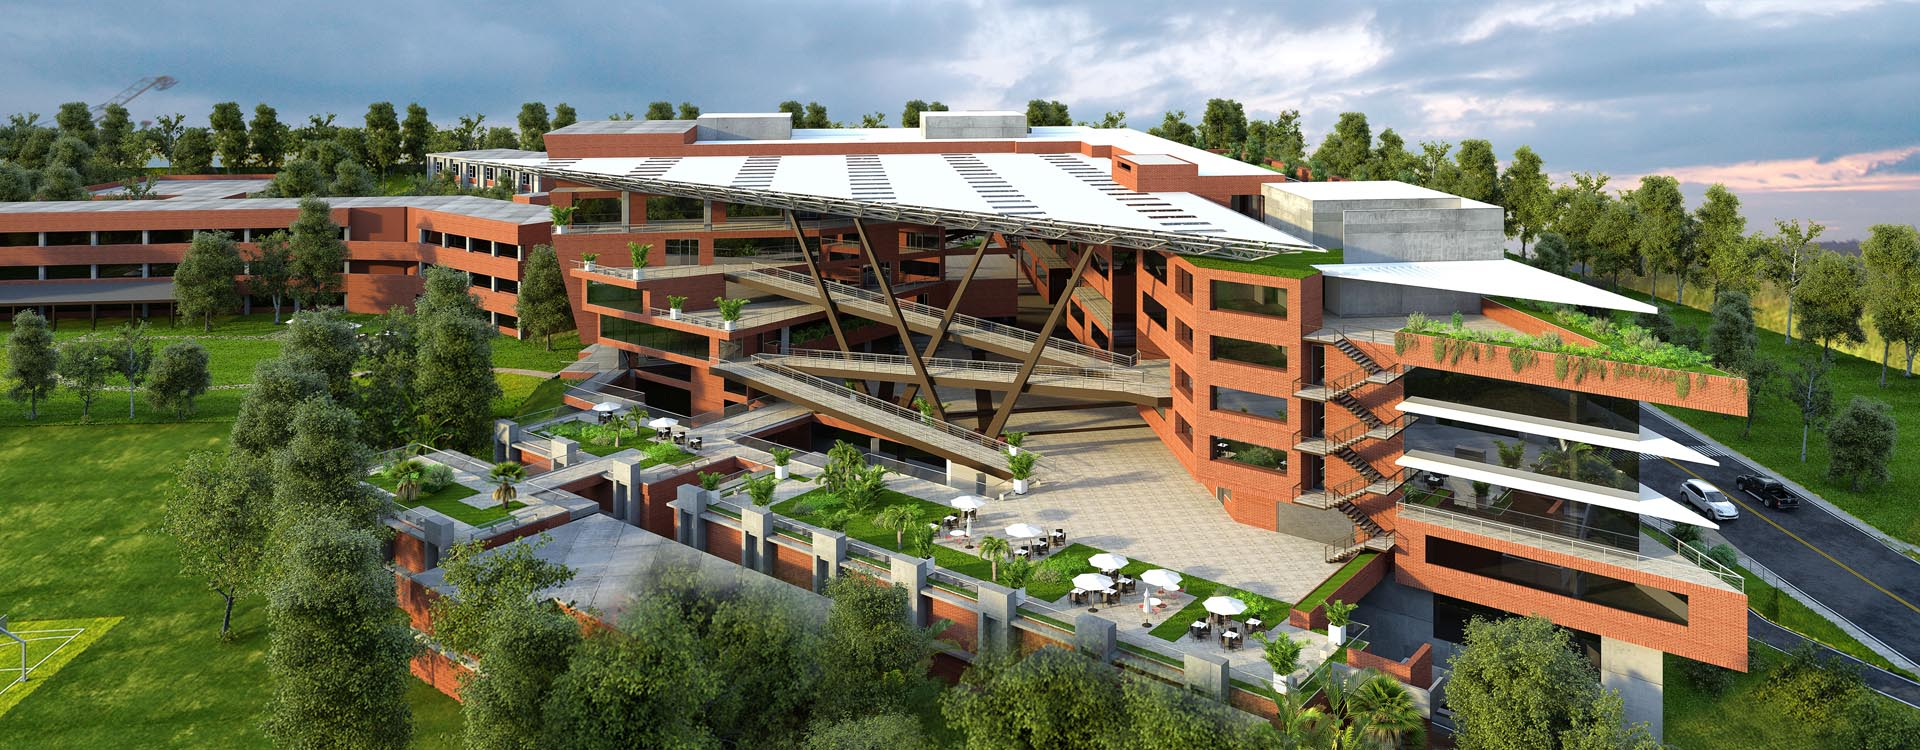
\includegraphics[height=13.25cm]{plantilla/portadacit.jpg}}
    	\makebox[\textwidth]{
    		\begin{overpic}[height=13.25cm]{\imagenportada}
     		\put(63,0){
\includegraphics[height=1.15in]{plantilla/fondologo_grande.png}}  
  			\put(64.5,2){
\includegraphics[height=0.55in]{plantilla/logoUVGblanco.eps}} 
        	\end{overpic}
    	}
    	%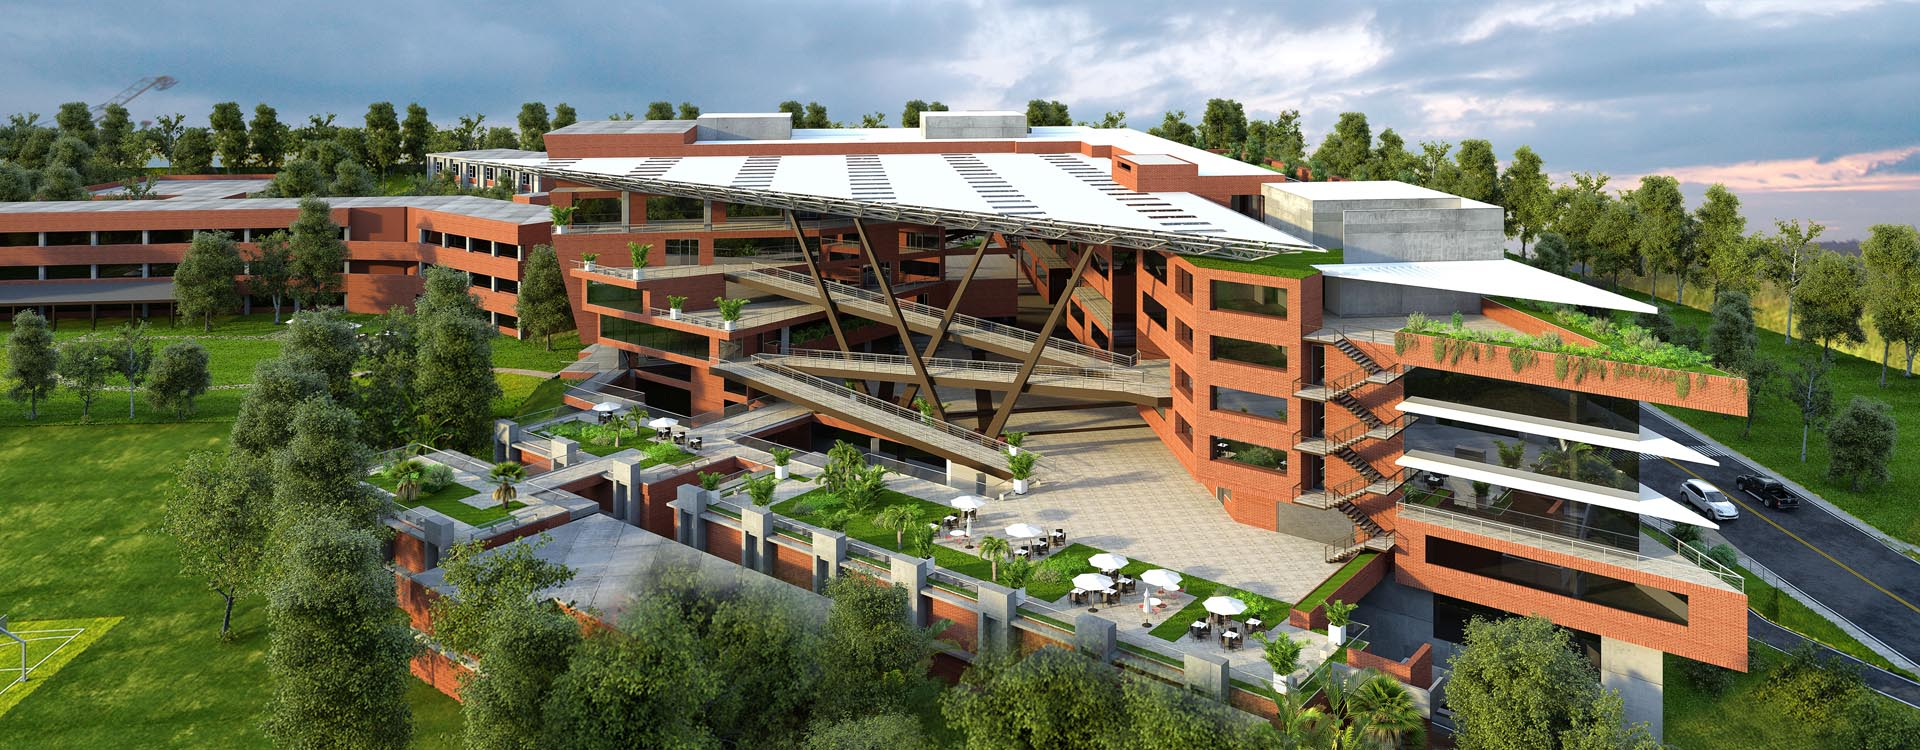
\includegraphics[height=13.25cm]{plantilla/portadacit.jpg}
	\end{figure}
	\restoregeometry
\fi

% ==============================================================================
% PRIMERAS PÁGINAS (Carátulas más hojas de guarda)
% ==============================================================================
\ifdefined\CAPcaratula
	\newpage
    \cleardoublepage\phantomsection
    % \pdfbookmark{Carátula}{toc}
	\pagecolor{white}
	\color{black}
	\setcounter{page}{1}
	\pagenumbering{roman}
	\thispagestyle{empty}
	\begin{center}
		\LARGE UNIVERSIDAD DEL VALLE DE GUATEMALA\\
		\LARGE Facultad de \uvgfacultad \\[0.75cm]
	\end{center}
	\begin{figure}[h]
		\begin{center}
		
\includegraphics[height=5.5 cm]{plantilla/escudoUVGnegro.eps}
		\vspace{0.5in}
		\end{center}
	\end{figure}
	\begin{center}
		\Large \textbf{\nohyphens{\titulotesis}} \\
		%\LARGE \textbf{\titulotesis} \\
		\vfill
		\Large \nohyphens{Trabajo de graduación presentado por \nombreestudiante \ para optar al grado académico de Licenciado en \uvgcarrera} \\
		\vfill
		\large Guatemala, \\
		\vspace{1em}
		\anoentrega
	\end{center}
    
    \ifdefined\printver	
	    \blankpage
	    \blankpage
	    
	    \newpage
	    \cleardoublepage\phantomsection
	    \pagecolor{white}
    	\color{black}
    	\setcounter{page}{1}
    	\pagenumbering{roman}
    	\thispagestyle{empty}
    	\begin{center}
    		\LARGE UNIVERSIDAD DEL VALLE DE GUATEMALA\\
    		\LARGE Facultad de \uvgfacultad \\[0.75cm]
    	\end{center}
    	\begin{figure}[h]
    		\begin{center}
    		
\includegraphics[height=5.5 cm]{plantilla/escudoUVGnegro.eps}
    		\vspace{0.5in}
    		\end{center}
    	\end{figure}
    	\begin{center}
    		\Large \textbf{\nohyphens{\titulotesis}} \\
    		%\LARGE \textbf{\titulotesis} \\
    		\vfill
    		\Large \nohyphens{Trabajo de graduación presentado por \nombreestudiante \ para optar al grado académico de Licenciado en \uvgcarrera} \\
    		\vfill
    		\large Guatemala, \\
    		\vspace{1em}
    		\anoentrega
    	\end{center}
    \fi
\fi

% ==============================================================================
% HOJA DE FIRMAS
% ==============================================================================
\ifdefined\CAPfirmas
	\newpage
	\cleardoublepage\phantomsection
	\thispagestyle{empty}
	\vspace*{0.5in}
	\large Vo.Bo.:\\[1cm]
	\begin{center}
		(f) \rule[1pt]{4 in}{1pt}\\
		\nombreasesor
	\end{center}
	\vspace{1in}

	Tribunal Examinador:\\[1cm]
	\begin{center}
		(f) \rule[1pt]{4 in}{1pt}\\
		\nombreasesor \\[1in]
		(f) \rule[1pt]{4 in}{1pt}\\
		\nombreprimerex \\[1in]
		(f) \rule[1pt]{4 in}{1pt}\\
		\nombresegundoex
	\end{center}
	\vspace{1in}

	Fecha de aprobación: Guatemala, \rule[1pt]{0.5 in}{1pt} de \rule[1pt]{1 in}{1pt} de \anoaprobacion.
	\normalsize
\fi

% Comentar para formato estilo libro en la numeración de páginas (NO 
% compatible con la guía UVG 2019)
\pagestyle{plain}
% ==============================================================================
% CONTENIDO DEL TRABAJO
% ==============================================================================
% DEDICATORIA
% ------------------------------------------------------------------------------
\ifdefined\CAPdedicatoria
	\newpage
	\cleardoublepage\phantomsection
    \chapter*{Dedicatoria}
    \ifdefined\parpordefecto
    	\defaultparformat{a-dedicatoria}
    \else
    	Plantilla dedicatoria
    \fi
    \addcontentsline{toc}{chapter}{Dedicatoria}
\fi
% PREFACIO
% ------------------------------------------------------------------------------
\ifdefined\CAPprefacio
	\newpage
	\cleardoublepage\phantomsection
    \chapter*{Prefacio}
    \ifdefined\parpordefecto
    	\defaultparformat{b-prefacio}
    \else
    	Lorem ipsum dolor sit amet, consectetur adipiscing elit. Cras vitae eleifend ipsum, ut mattis nunc. Pellentesque ac hendrerit lacus. Cras sollicitudin eget sem nec luctus. Vivamus aliquet lorem id elit venenatis pellentesque. Nam id orci iaculis, rutrum ipsum vel, porttitor magna. Etiam molestie vel elit sed suscipit. Proin dui risus, scelerisque porttitor cursus ac, tempor eget turpis. Aliquam ultricies congue ligula ac ornare. Duis id purus eu ex pharetra feugiat. Vivamus ac orci arcu. Nulla id diam quis erat rhoncus hendrerit. Class aptent taciti sociosqu ad litora torquent per conubia nostra, per inceptos himenaeos. Sed vulputate, metus vel efficitur fringilla, orci ex ultricies augue, sit amet rhoncus ex purus ut massa. Nam pharetra ipsum consequat est blandit, sed commodo nunc scelerisque. Maecenas ut suscipit libero. Sed vel euismod tellus.

Proin elit tellus, finibus et metus et, vestibulum ullamcorper est. Nulla viverra nisl id libero sodales, a porttitor est congue. Maecenas semper, felis ut rhoncus cursus, leo magna convallis ligula, at vehicula neque quam at ipsum. Integer commodo mattis eros sit amet tristique. Cras eu maximus arcu. Morbi condimentum dignissim enim non hendrerit. Sed molestie erat sit amet porttitor sagittis. Maecenas porttitor tincidunt erat, ac lacinia lacus sodales faucibus. Integer nec laoreet massa. Proin a arcu lorem. Donec at tincidunt arcu, et sodales neque. Morbi rhoncus, ligula porta lobortis faucibus, magna diam aliquet felis, nec ultrices metus turpis et libero. Integer efficitur erat dolor, quis iaculis metus dignissim eu.
    \fi
    \addcontentsline{toc}{chapter}{Prefacio}
\fi

% RESUMEN
% ------------------------------------------------------------------------------
\ifdefined\CAPresumen
	\newpage
    \cleardoublepage\phantomsection
	\chapter*{Resumen}
	\ifdefined\parpordefecto
		\defaultparformat{c-resumen}
	\else
		La inteligencia artificial (IA) ofrece un potencial transformador para la educación, especialmente en contextos marcados por desigualdades sociales, económicas y tecnológicas. En países como Guatemala, donde persiste una amplia brecha educativa, la IA puede convertirse en una herramienta clave para facilitar el acceso a aprendizajes significativos.

Uno de los ámbitos más desatendidos es la formación ciudadana y el desarrollo de valores morales, que, aunque incluidos en los programas educativos, suelen abordarse de forma teórica y desvinculada de la realidad social. Es aquí donde se plantea la importancia de una herramienta que brinde acompañamiento a los estudiantes en la reflexión sobre su papel como ciudadanos y en la práctica de valores como el respeto, la empatía y la responsabilidad, un proyecto que combine tanto la tecnología accesible como un enfoque centrado en el usuario para fortalecer no solo el aprendizaje, sino también la conciencia social y ética de los jóvenes.

La implementación de esta herramienta contempla la digitalización de contenidos educativos, el desarrollo de un modelo de IA adaptado al contexto local y finalmente la validación directa
de la interacción con la herramienta para verificar que las respuestas dadas coincidan con el material proporcionado. Como resultado, se busca una solución funcional, innovadora y escalable que demuestre cómo la IA puede contribuir significativamente al fortalecimiento de la educación en valores en entornos con recursos limitados.
	\fi
	\addcontentsline{toc}{chapter}{Resumen}
\fi

% ABSTRACT
% ------------------------------------------------------------------------------
\ifdefined\CAPabstract
	\newpage
    \cleardoublepage\phantomsection
	\chapter*{Abstract}
	\ifdefined\parpordefecto
		\defaultparformat{d-abstract}
	\else
		Artificial intelligence (AI) offers transformative potential for education, especially in contexts marked by social, economic, and technological inequalities. In countries like Guatemala, where a wide educational gap persists, AI can become a key tool to facilitate access to meaningful learning.

One of the most neglected areas is civic education and the development of moral values, which, although included in educational programs, are often addressed theoretically and detached from social reality. It is here that the importance of a tool that provides support to students in reflecting on their role as citizens and in the practice of values such as respect, empathy, and responsibility arises, a project that combines both accessible technology and a user-centered approach to strengthen not only learning, but also the social and ethical awareness of young people.

The implementation of this tool contemplates the digitization of educational content, the development of an AI model adapted to the local context, and finally, the direct validation of the interaction with the tool to verify that the answers given match the material provided. As a result, a functional, innovative, and scalable solution is sought that demonstrates how AI can significantly contribute to the strengthening of values education in environments with limited resources.
	\fi
	\addcontentsline{toc}{chapter}{Abstract}
\fi

% ÍNDICE GENERAL
% ------------------------------------------------------------------------------
\ifdefined\CAPindice
	\newpage
    \cleardoublepage\phantomsection
	\renewcommand{\contentsname}{Índice}
    %\phantomsection
    \pdfbookmark{\contentsname}{toc}
    %\pdfbookmark{Índice}{toc}
	\tableofcontents
\fi

% LISTADO DE CUADROS
% ------------------------------------------------------------------------------
\ifdefined\CAPcuadros
\newpage
\cleardoublepage\phantomsection
\renewcommand{\listtablename}{Lista de cuadros}
\listoftables
\addcontentsline{toc}{chapter}{Lista de cuadros}
\fi

% LISTADO DE FIGURAS
% ------------------------------------------------------------------------------
\ifdefined\CAPfiguras
	\newpage
    \cleardoublepage\phantomsection
	\renewcommand{\listfigurename}{Lista de figuras}
	\listoffigures
	\addcontentsline{toc}{chapter}{Lista de figuras}
\fi

% GLOSARIO
% ------------------------------------------------------------------------------
\ifdefined\CAPglosario
	\newpage
	\printglossary
\fi

% INTRODUCCIÓN
% ------------------------------------------------------------------------------
\ifdefined\CAPintroduccion
	\newpage
	\cleardoublepage
	\pagenumbering{arabic}
	\setcounter{page}{1}
	\chapter{Introducción}
	\ifdefined\parpordefecto
		\defaultparformat{f-introduccion}
	\else
		La formación en valores y ciudadanía constituye un componente fundamental en la construcción de sociedades democráticas, inclusivas y participativas. A través de ella, los estudiantes desarrollan competencias cívicas como la empatía, la responsabilidad social, el respeto a la diversidad y el compromiso con el bien común. Diversos organismos internacionales, como la UNESCO y la OCDE, han destacado la importancia de reforzar estos aprendizajes en contextos educativos cada vez más desafiantes, marcados por tensiones sociales, crisis ambientales y transformaciones digitales profundas \cite{unesco2021ethics,oecd2021skills}. No obstante, en muchos países de América Latina, esta dimensión formativa continúa siendo relegada frente a enfoques centrados únicamente en resultados académicos medibles \cite{worldbank2022revolution,rivas2023future}.

En el caso de Guatemala, si bien el Currículo Nacional Base reconoce la educación ciudadana como un eje transversal, su aplicación efectiva enfrenta múltiples obstáculos; como la falta de metodologías activas, el uso limitado de recursos digitales y la escasa formación docente en enfoques críticos y reflexivos. Estas condiciones dificultan que los estudiantes puedan vincular los contenidos cívicos con sus experiencias cotidianas o desarrollar una comprensión profunda de su papel como agentes de cambio en sus comunidades \cite{mineduc2020cnb,cien2019diagnostico}. A ello se suma una brecha tecnológica significativa entre zonas urbanas y rurales, lo cual limita las oportunidades para introducir enfoques innovadores que promuevan aprendizajes significativos en valores y ciudadanía \cite{unesco2023monitoring,levy2025teachers}.

Ante este escenario, la inteligencia artificial (IA) se presenta como una herramienta con potencial transformador en el ámbito educativo, particularmente cuando se orienta hacia el fortalecimiento de habilidades humanas y no únicamente hacia la automatización de contenidos. La UNESCO ha enfatizado que, para que estas tecnologías contribuyan a sistemas educativos más justos y democráticos, deben diseñarse bajo principios de equidad, inclusión y supervisión humana, evitando reproducir sesgos o exclusiones preexistentes \cite{unesco2021ethics,unesco2021guidance}. Aplicada con criterio ético y pedagógico, la IA puede ser utilizada como un recurso para ampliar el acceso a materiales formativos, personalizar la experiencia de aprendizaje y acompañar procesos de reflexión moral desde una lógica de diálogo \cite{frontiers2024chatgpt,tulsiani2024chatgpt}.

En base a todo lo expuesto, la solución propuesta consiste en un sistema basado en un modelo |de lenguaje (LLM) apoyado en una base de datos vectorial que almacena documentos éticos, pedagógicos y contextuales mediante técnicas de embedding. Este tutor virtual, accesible desde dispositivos de bajo costo y alta accesibilidad, genera respuestas personalizadas y fundamentadas que acompañan el aprendizaje informal en valores y ciudadanía, estimulando la reflexión crítica y la toma de decisiones éticas. Más que sustituir al docente, este sistema busca potenciar la iniciativa del estudiante, ofreciendo un recurso inclusivo que aporte un acompañamiento directo en su día a día, diseñado en base a material validado por profesionales expertos para asegurar un enfoque humanizado y contextualizado a las realidades actuales del país \cite{unesco2021ethics,worldbank2022revolution,rivas2023future}.
	\fi
\fi

% JUSTIFICACIÓN
% ------------------------------------------------------------------------------
\ifdefined\CAPjustificacion
	\newpage
	\chapter{Justificación}
	\ifdefined\parpordefecto
		\defaultparformat{g-justificacion}
	\else
		La llegada de modelos conversacionales, como ChatGPT, ha revolucionado el aprendizaje, permitiendo tutorías personalizadas que adaptan el contenido al ritmo del estudiante y ofrecen retroalimentación inmediata, factores clave para mejorar la motivación y el rendimiento académico en contextos diversos \cite{frontiers2024chatgpt}. Sin embargo, investigaciones advierten sobre riesgos como la desinformación o el plagio si estos sistemas se emplean sin supervisión pedagógica, lo que subraya la necesidad de un diseño ético y guiado \cite{tulsiani2024chatgpt}. Además, la inteligencia artificial (IA) está transformando la gestión educativa al automatizar tareas administrativas como la calificación de exámenes y el seguimiento de asistencia, liberando tiempo para que los docentes se centren en procesos pedagógicos de mayor valor \cite{unesco2023monitoring}.

En América Latina, las plataformas de IA están extendiendo recursos digitales a zonas rurales, reduciendo brechas de cobertura; sin embargo, su escalabilidad sigue limitada por deficiencias en infraestructura y falta de formación técnica docente \cite{worldbank2022revolution,rivas2023future}. En el caso de Guatemala, el Acuerdo Ministerial 2810-2023 estableció el Programa Nacional de Educación en Valores para priorizar la formación ciudadana \cite{mineduc2023acuerdo}, aunque el Diagnóstico del CIEN, realizado en 2019 evidenció problemas persistentes en cobertura, eficiencia, calidad y ausencia de estrategias de tecnología educativa \cite{cien2019diagnostico}.

En este contexto, los modelos de lenguaje (LLMs) ofrecen una propuesta tecnológica altamente pertinente, en este caso, como tutores en valores y ciudadanía. Su capacidad para imitar patrones de diálogo humano, que incluyen desde el ajuste del tono al hablar hasta el nivel de complejidad, facilita interacciones conversacionales continuas que se acoplan al contexto que se esté tratando, similar a como lo haría un tutor humano para con el estudiante \cite{qin2024transforming}. Diversos estudios han demostrado que los LLMs pueden fomentar la auto-reflexión y el pensamiento crítico mediante estrategias como el método Socrático que, en algunos casos, alcanzan e incluso llegan a superar niveles de efectividad comparables a cuestionarios estructurados \cite{cordova2025aiagents}. En particular, la técnica de Retrieval-Augmented Generation (RAG), permite que los LLMs fundamenten sus respuestas en documentos específicos (por ejemplo, guías curriculares, casos de estudio resueltos), de manera que se reducen enormemente las respuestas imaginadas por la IA, a la vez que se mejora la confianza en la herramienta \cite{cordova2025aiagents,levonian2025safechats}.

Los LLMs, por tanto, se diferencian de otras herramientas de IA al ofrecer una tutoría que se adapta al estilo de aprendizaje y comprensión del estudiante, ofrece retroalimentación inmediata, y mantiene el diálogo necesario para estimular el juicio ético en casos de la vida cotidiana del estudiante; todo ello sin pretender sustituir la educación tradicional, sino complementando el aprendizaje teórico al permitir que el estudiante fortalezca su rol como ciudadano en el día a día. Para asegurar que este sistema contribuya a reducir en lugar de profundizar brechas, es necesario entrenarlo con materiales éticos y contextuales, y mantener supervisión continua por educadores y profesionales en el área \cite{unesco2021ethics,unesco2021guidance}. Estas condiciones permiten generar interacciones fundamentadas y culturalmente pertinentes, garantizando una tutoría ética y efectiva en valores y ciudadanía.
	\fi
\fi

% ANTECEDENTES
% ------------------------------------------------------------------------------
\ifdefined\CAPantecedentes
	\newpage
	\chapter{Antecedentes}
	\ifdefined\parpordefecto
    	\defaultparformat{h-antecedentes}
    \else
    	Puede encontrarse un trabajo similar en \cite{hoover2010bio} o bien \cite{park2014design}
    \fi  
\fi

% OBJETIVOS
% ------------------------------------------------------------------------------
\ifdefined\CAPobjetivos
	\newpage
	\chapter{Objetivos}
	\ifdefined\parpordefecto
		\defaultparformat{i-objetivos}
	\else
		\section{Objetivo general}
Desarrollar una herramienta tecnológica de educación informal orientada al acompañamiento en la adquisición de aprendizajes sobre formación ciudadana y valores morales.

\section{Objetivos específicos}
\begin{itemize}
\item Implementar un modelo LLM pre-entrenado y optimizado para obtener respuestas coherentes y acordes a la solicitud del usuario.
\item Integrar una base de datos vectorial para almacenar y recuperar información actualizada que proporcione respuestas fundamentadas en el contenido preseleccionado.
\item Desarrollar una interfaz gráfca atractiva para dispositivos móviles que permita la interacción entre el usuario y el modelo de inteligencia artifcial.
\end{itemize}
	\fi
\fi

% ALCANCE
% ------------------------------------------------------------------------------
\ifdefined\CAPalcance
	\newpage
	\chapter{Alcances}
	\ifdefined\parpordefecto
    	\defaultparformat{j-alcance}
    \else
    	Podemos usar \Gls{latex} para escribir de forma ordenada una \gls{formula} matemática. 
    \fi 
\fi

% MARCO TEÓRICO
% ------------------------------------------------------------------------------
\ifdefined\CAPmarcoteorico
	\newpage
	\chapter{Marco teórico}
	\ifdefined\parpordefecto
		\defaultparformat{k-marco_teorico}
	\else
		Aunque a primera vista puedan parecer ámbitos completamente distintos, la
formación en valores y la inteligencia artificial (IA) convergen hoy como una
de las propuestas más innovadoras dentro del campo educativo. La incorporación
de sistemas inteligentes ha comenzado a transformar las prácticas de enseñanza
y aprendizaje, tanto en el nivel formal como informal. En la educación formal,
ya se evidencian los efectos del uso de asistentes basados en IA por parte de
estudiantes y docentes: los primeros los utilizan para investigar, estructurar
tareas o practicar ejercicios, mientras que los segundos los emplean para
generar materiales, personalizar recursos didácticos y optimizar procesos de
evaluación \cite{elstad2024ai, frontiers2025education}.

No obstante, en un contexto global caracterizado por aceleradas
transformaciones tecnológicas y crecientes tensiones sociales, la formación
ciudadana adquiere una relevancia urgente. Las metodologías tradicionales
requieren ser replanteadas a la luz de las nuevas herramientas digitales, sin
perder su esencia formativa: desarrollar personas críticas, éticas y
responsables capaces de convivir en armonía y contribuir activamente a su
entorno \cite{betterinternet2024}. En este sentido, el acompañamiento educativo
informal mediante medios digitales surge como una oportunidad complementaria
para guiar a los jóvenes en la toma de decisiones morales y sociales,
proporcionándoles una orientación accesible y contextualizada
\cite{carter2024ethics, seibt2024llm}.

Desde esta perspectiva, resulta pertinente integrar la formación ciudadana con
tecnologías emergentes como los modelos de lenguaje de gran escala (LLM). Estas
herramientas, cuando se diseñan con criterios éticos y pedagógicos, pueden
favorecer el desarrollo del pensamiento crítico, la reflexión moral y la
educación en valores dentro de entornos digitales. Además, permiten ofrecer
acompañamiento educativo personalizado y continuo, promoviendo un aprendizaje
significativo y responsable \cite{frontiers2025psychology, elstad2024ai}. En
consecuencia, se plantea el desarrollo de una solución tecnológica basada en IA
que sirva como acompañante educativo informal, orientada a fortalecer la
educación ciudadana y los valores en la era digital, procurando un equilibrio
entre innovación, pertinencia social y responsabilidad ética.

\section{Educación ciudadana y valores}
La educación ciudadana constituye un proceso educativo integral orientado a
formar individuos capaces de ejercer sus derechos y deberes de manera
responsable, ética y crítica. Esta formación no se limita al conocimiento de
normas y leyes, sino que promueve valores como la solidaridad, la justicia y el
respeto por la diversidad, esenciales para la convivencia democrática
\cite{unesco2021global, torney2007civic}. Además, la educación ciudadana
incorpora competencias sociales y habilidades de pensamiento crítico,
fomentando la participación activa en la comunidad y la toma de decisiones
informadas \cite{bentley2018education}.

\subsection{Educación en valores}
La educación en valores constituye un enfoque pedagógico reconocido a nivel
internacional bajo diversas denominaciones, como educación moral, educación del
carácter o educación ética. Si bien cada una presenta matices particulares y
distintos énfasis, todas comparten la convicción fundamental de que la
formación en valores personales y cívicos representa una responsabilidad
legítima de las instituciones educativas a nivel mundial. En la actualidad,
este ámbito ya no se considera exclusivo del entorno familiar o religioso, pues
diversas investigaciones han evidenciado que una educación desvinculada de los
valores puede limitar de forma significativa el desarrollo integral del
estudiante, tanto en el plano ético como en el académico.\cite{lovat2009values}

Asimismo, la educación en valores se concibe como un proceso formativo integral
que no solo promueve principios fundamentales de ética y ciudadanía, sino que
se posiciona como un componente esencial y transversal de la calidad educativa.
Lejos de tratarse de un aspecto aislado, establece una relación de mutua
interdependencia con la enseñanza de calidad, al punto de integrarse en una
dinámica de doble hélice que potencia el desarrollo personal, social y
académico del estudiante. \cite{lovat2009values}

\subsection{Formación ciudadana}
La formación ciudadana, bajo el concepto anglosajón de civic education, es el
conjunto de procesos, formales e informales, mediante los cuales las personas
desarrollan conocimientos, valores, actitudes, habilidades y compromisos que
les permiten participar activamente y de manera crítica en la vida democrática
y comunitaria; éste no está limitado al ámbito escolar ni a una etapa
específica de la vida del individuo, sino que se extiende a lo largo de su
ciclo vital e involucra diversos aspectos externos como la familia, los medios
de comunicación, su comunidad, instituciones educativas, etc.
\cite{crittenden2007civic}

Por lo tanto, la formación ciudadana no se limita a la transmisión de
contenidos normativos sobre el sistema político, sino que incorpora prácticas
educativas activas, como la discusión de temas controversiales, la
participación en acciones colectivas y la reflexión crítica, las cuales han
demostrado tener efectos significativos en el desarrollo de una ciudadanía
activa, consciente y empoderada. \cite{crittenden2007civic}

\subsection{Competencias cívicas fundamentales}
Las competencias cívicas fundamentales son un conjunto integrado de
disposiciones personales y capacidades que permiten a los individuos participar
activamente en sociedades democráticas diversas. De acuerdo con el Consejo de
Europa, estas competencias se organizan en torno a cuatro dimensiones
esenciales: los valores que guían el comportamiento ético; las actitudes que
predisponen a la apertura y al respeto; las habilidades necesarias para la
interacción democrática; y los conocimientos y la comprensión crítica del mundo
social, político y cultural. Su desarrollo es clave para convivir como iguales
en contextos diversos y democráticos. \cite{barrett2016competences}

\subsubsection{Valores}
Los valores son creencias fundamentales que orientan a las personas hacia metas
que consideran deseables en la vida. Funcionan como motores de acción y como
criterios que guían la toma de decisiones, al proporcionar marcos de referencia
sobre lo que se considera apropiado pensar o hacer en diversas situaciones.
Estos principios no se limitan a contextos específicos, sino que ofrecen
estándares para evaluar conductas, justificar posturas, elegir entre opciones,
planificar acciones e influir en otros. \cite{barrett2016competences}

\subsubsection{Actitudes}
Las actitudes representan la disposición mental general que una persona adopta
frente a individuos, grupos, instituciones, temas u objetos simbólicos. Esta
orientación suele estar compuesta por cuatro elementos interrelacionados: una
creencia o juicio cognitivo sobre el objeto, una respuesta emocional, una
valoración positiva o negativa, y una inclinación conductual específica hacia
dicho objeto. \cite{barrett2016competences}

\subsubsection{Habilidades}
Las habilidades son capacidades que permiten organizar y ejecutar de forma
eficiente patrones complejos de pensamiento o acción, adaptándolos al contexto
con el propósito de alcanzar un objetivo específico.
\cite{barrett2016competences}

\subsubsection{Conocimientos y Comprensión Crítica}
Los conocimientos representan el conjunto de información que una persona ha
adquirido, mientras que la comprensión crítica implica no solo entender esa
información, sino también valorar de forma reflexiva los sentimientos,
perspectivas y significados asociados a ella. Este tipo de comprensión es
esencial en contextos democráticos e interculturales, ya que permite analizar e
interpretar activamente las situaciones, superando respuestas automáticas o no
conscientes. En ese sentido, favorece la evaluación crítica de lo que se sabe y
de cómo se interpreta el mundo social y político. \cite{barrett2016competences}

\subsection{Educación moral}
La educación moral es el proceso educativo centrado en la moralidad, entendida
principalmente como la adhesión a normas morales y la creencia en su
justificación. Este enfoque puede implicar dos dimensiones fundamentales: por
un lado, la formación moral, que busca desarrollar en los individuos
disposiciones afectivas, conductuales y motivacionales alineadas con esas
normas; y por otro, la indagación moral, que promueve la reflexión crítica yla
construcción de creencias fundamentadas sobre la validez de dichas normas.
Ambas dimensiones pueden ser abordadas de manera complementaria, aunque
conceptualmente son distintas. Además, el autor reconoce que la moralidad
podría abarcar elementos adicionales, como ciertas virtudes o disposiciones
emocionales, cuya formación también puede formar parte significativa de la
educación moral. \cite{hand2017moral}

\subsubsection{Formación Moral}
La formación moral es una dimensión de la educación moral centrada en el
desarrollo de disposiciones afectivas y conductuales que llevan a una persona a
adherirse a normas morales y a responder emocionalmente a ellas. No se trata
únicamente de enseñar qué está bien o mal, sino de fomentar inclinaciones
internas que impulsen a actuar conforme a ciertos estándares, de forma estable
y espontánea. Estas disposiciones pueden incluir sentimientos de satisfacción
cuando se actúa moralmente, incomodidad al violar principios morales, y
expectativas de que otros también se comporten moralmente. \cite{hand2017moral}

Asimismo, este concepto puede abarcar el cultivo de virtudes, entendidas no
solo como inclinaciones a seguir normas, sino como capacidades para moderar
emociones humanas fundamentales. Bajo esta perspectiva, la formación moral no
se reduce a enseñar reglas, sino que apunta a moldear el carácter y las
emociones de forma que apoyen una vida moral.\cite{hand2017moral}

\subsubsection{Indagación Moral}
La indagación moral es la parte de la educación moral que se enfoca en
investigar y evaluar la justificación de las normas morales. Consiste en un
proceso cognitivo mediante el cual se analiza por qué una norma debería ser
aceptada, se examinan los argumentos que la sustentan y se reflexiona
críticamente sobre ellos. Creer en la justificación de una norma no es un
requisito para adherirse a ella, por lo que esta indagación es distinta de la
formación moral, que busca cultivar la adhesión emocional y conductual a esas
normas. \cite{hand2017moral}

En la enseñanza de la indagación moral, es posible adoptar un enfoque
directivo, orientando al individuo hacia una conclusión particular sobre la
validez de una norma, o un enfoque no directivo, en el que se facilita el
análisis y la discusión sin influir en la opinión final. Ambos métodos
promueven la capacidad del individuo para pensar críticamente sobre las normas
morales y su justificación, complementando así la formación moral.
\cite{hand2017moral}

\section{Aprendizaje informal y brecha educativa}
El aprendizaje informal constituye una estrategia educativa que ocurre fuera de
los entornos formales, como escuelas o universidades, y se produce de manera
espontánea en la vida cotidiana. Este tipo de educación fomenta la autonomía
del aprendiz, la creatividad y la resolución de problemas, contribuyendo a
reducir la brecha educativa, especialmente cuando el acceso a la educación
formal es limitado \cite{coombs1968world, mills2014informal}.

\subsection{Educación informal}
La educación informal se refiere a las formas de aprendizaje que ocurren de
manera natural en la vida cotidiana, en una amplia variedad de contextos
geográficos e históricos. Este tipo de educación no se limita a entornos
específicos, sino que suele surgir en espacios dondelas personas se sienten
cómodas y con la libertad de socializar entre sí. Aunque este concepto es
asociado tradicionalmente con actividades fuera de la escuela, hoy en día la
educación informal también puede darse dentro de escuelas convencionales o en
organizaciones como el voluntariado juvenil o el movimiento scout.
\cite{mills2014informal}

Este tipo de educación se basa en el diálogo y la conversación, fomentando la
confianza, el respeto y la empatía. No busca imponer resultados específicos,
sino que promueve el aprendizaje a partir de las preocupaciones reales y
cotidianas de las personas, generando cambios positivos y significativos en sus
vidas. Además, la educación informal puede tener un carácter político,
inspirándose en enfoques críticos que buscan que las personas tomen conciencia
de las injusticias sociales y encuentren formas de superarlas, conectando lo
personal con temas sociales y políticos más amplios. \cite{mills2014informal}

\subsection{Autoformación guiada}
La autoformación guiada es un proceso intencional en el que el sujeto
desarrolla su aprendizaje autónomo con el apoyo de una institución, un educador
o un colectivo social. Aunque el aprendiz asume responsabilidad sobre sus
objetivos, recursos, métodos y ritmos, recibe orientación y acompañamiento que
facilitan el desarrollo de su capacidad de aprendizaje y auto-regulación.
\cite{Dumazedier1998}

En este enfoque, la autoformación deja de ser un esfuerzo completamente
solitario o espontáneo para convertirse en una práctica educacional
estructurada, donde la ayuda externa configura las condiciones que permiten que
el sujeto social desarrolle su propio proyecto formativo y consolide su agencia
como aprendiz activo en su entorno social. \cite{Dumazedier1998}

\subsection{Brecha educativa y tecnológica}
La brecha educativa y tecnológica se refiere a las diferencias en el acceso y
aprovechamiento de recursos educativos y tecnológicos entre distintos grupos
sociales. Estas desigualdades afectan la calidad del aprendizaje, limitan la
participación en entornos digitales y pueden amplificar la exclusión social.
Factores como el acceso desigual a internet, dispositivos digitales y
capacitación docente contribuyen a esta brecha, la cual requiere estrategias
integrales de inclusión digital \cite{van2005digital, warschauer2011learning}.

\subsection{Tecnología como herramienta de inclusión educativa}
La tecnología educativa se ha consolidado como una herramienta estratégica para
promover la inclusión educativa, al facilitar el acceso a contenidos y recursos
didácticos a estudiantes con diversidad de contextos, habilidades y
necesidades. Plataformas digitales, dispositivos móviles y herramientas de
aprendizaje asistidas por inteligencia artificial permiten superar barreras
geográficas, socioeconómicas y culturales, mejorando la equidad en la educación
\cite{selwyn2016education, unicef2019digital}.

\section{Inteligencia Artificial y método socrático digital}
La inteligencia artificial (IA) aplicada a la educación ofrece oportunidades
para diseñar entornos de aprendizaje interactivos y personalizados. Una de las
estrategias más prometedoras es la implementación de métodos socráticos
digitales, donde los sistemas de IA guían a los estudiantes mediante preguntas
y diálogos reflexivos, estimulando el pensamiento crítico y la autonomía en la
construcción del conocimiento \cite{holmes2019ai, graesser2021ai}.

\subsection{Inteligencia Artificial en la educación}
La IA en la educación permite automatizar tareas administrativas, ofrecer
tutorías personalizadas, monitorear el progreso de los estudiantes y adaptar
los contenidos a sus necesidades individuales. Estas aplicaciones han
demostrado mejorar la motivación, la eficiencia del aprendizaje y la calidad de
la enseñanza, siempre que se acompañen de supervisión pedagógica y criterios
éticos claros \cite{elstad2024ai, frontiers2025education, carter2024ethics}.

\subsection{Modelos de Lenguaje de Gran Escala (LLMs)}
Los modelos de lenguaje de gran escala (LLMs) son sistemas de inteligencia
artificial entrenados con enormes volúmenes de texto para comprender y generar
lenguaje natural. Estos modelos permiten ofrecer respuestas contextualizadas,
realizar tutorías personalizadas y asistir en la construcción de conocimiento
mediante diálogo interactivo. Su potencial educativo radica en la capacidad de
proporcionar retroalimentación inmediata, adaptada al nivel del estudiante,
fomentando la reflexión crítica y la autoformación \cite{brown2020language,
    raffel2020exploring}.

\subsection{Recuperación aumentada por búsqueda (RetrievalAugmented Generation, RAG)}
La Recuperación Aumentada por Búsqueda (RAG) combina modelos de lenguaje con
motores de búsqueda para proporcionar información precisa y contextualizada. En
educación en valores, esta técnica permite que los estudiantes reciban
respuestas fundamentadas en fuentes confiables, promoviendo la reflexión ética
y la resolución de dilemas morales basados en evidencia. RAG amplía las
capacidades de tutoría digital al integrar conocimiento externo con generación
de lenguaje natural \cite{lewis2020retrieval, khandelwal2020generalization}.

\subsection{Embeddings y representación vectorial del texto}
Los embeddings son representaciones vectoriales de palabras, frases o
documentos que capturan sus significados semánticos. Esta técnica permite que
los sistemas de IA comparen y recuperen información de manera eficiente,
midiendo la similitud entre conceptos y facilitando búsquedas semánticas. En
educación, los embeddings permiten vincular preguntas de los estudiantes con
contenidos relevantes, apoyando la personalización del aprendizaje
\cite{mikolov2013efficient, le2014distributed}.

\subsection{Bases de datos vectoriales y búsqueda semántica}
Las bases de datos vectoriales permiten almacenar y consultar embeddings de
manera eficiente, habilitando la búsqueda semántica en grandes volúmenes de
información. Este enfoque supera las limitaciones de las búsquedas basadas en
palabras clave, permitiendo que los estudiantes y sistemas educativos accedan a
contenidos relevantes de manera más precisa y contextualizada, facilitando la
recuperación de conocimiento en entornos digitales \cite{johnson2019billion,
    bernhard2022vector}.

\subsection{Método socrático aplicado a entornos digitales}
Los entornos digitales permiten implementar el método socrático mediante
sistemas de IA que guían a los estudiantes a través de preguntas reflexivas y
secuencias de razonamiento. Esta estrategia fomenta el pensamiento crítico y la
autonomía, ya que los alumnos deben analizar, argumentar y evaluar sus propias
respuestas antes de recibir retroalimentación. El uso de chatbots y asistentes
inteligentes basados en este método facilita un aprendizaje personalizado y
continuo, replicando la interacción dialógica propia del enfoque socrático
tradicional \cite{graesser2021ai, fox2020socratic}.

\subsection{Tutoría personalizada con IA}
La tutoría personalizada con IA permite adaptar los contenidos y las
estrategias de enseñanza al nivel, intereses y ritmo de cada estudiante. Los
sistemas inteligentes analizan patrones de aprendizaje y ofrecen
retroalimentación inmediata, identificando áreas de dificultad y recomendando
recursos específicos. Esta personalización mejora la motivación, la retención
de conocimiento y promueve la autonomía del aprendiz \cite{woolf2010building,
    duffy2019personalized}.

\subsection{Supervisión pedagógica en sistemas automatizados}
A pesar de la autonomía de los sistemas de IA, la supervisión pedagógica es
esencial para garantizar la calidad del aprendizaje. Docentes y tutores deben
monitorear el funcionamiento de los sistemas automatizados, evaluar la
relevancia y exactitud de las respuestas generadas, y ajustar los parámetros de
personalización según las necesidades de los estudiantes. Este enfoque mixto
asegura que la tecnología complemente, y no reemplace, la guía educativa
\cite{holmes2019ai, luckin2016intelligence}.

\section{Ética en IA educativa}
La ética en IA educativa aborda la responsabilidad en el diseño, implementación
y uso de sistemas inteligentes en contextos de aprendizaje. Incluye
consideraciones sobre privacidad de los datos, equidad, transparencia,
inclusión y impacto social. Garantizar que los estudiantes sean tratados de
manera justa y que los sistemas no reproduzcan sesgos existentes es crucial
para la confianza y efectividad de la educación asistida por IA
\cite{selwyn2019should, williamson2021ethics}.

\subsection{Principios éticos fundamentales en IA}
Los principios éticos fundamentales en IA incluyen transparencia, justicia, no
discriminación, responsabilidad, privacidad y seguridad. En el ámbito
educativo, estos principios guían el desarrollo de sistemas que respeten la
dignidad del estudiante, promuevan equidad en el aprendizaje y faciliten la
rendición de cuentas por parte de desarrolladores y educadores. La aplicación
de estos principios permite aprovechar el potencial de la IA sin comprometer la
integridad pedagógica \cite{jobin2019global, floridi2018ai}.

\subsection{Prevención de sesgos algorítmicos}
La prevención de sesgos algorítmicos se centra en garantizar que los sistemas
de IA no reproduzcan ni amplifiquen desigualdades existentes en la educación.
Esto implica analizar los datos de entrenamiento, identificar posibles sesgos y
aplicar técnicas de mitigación, como ajuste de ponderaciones, diversificación
de datasets y pruebas de equidad en los resultados. La prevención de sesgos
asegura que todos los estudiantes reciban oportunidades de aprendizaje justas y
equitativas \cite{mehrabi2019survey, binns2018fairness}.

\subsection{Transparencia y explicabilidad en sistemas inteligentes}
La transparencia y explicabilidad son fundamentales para que docentes,
estudiantes y desarrolladores comprendan cómo un sistema de IA toma decisiones.
Esto incluye técnicas de interpretabilidad que permitan visualizar la lógica de
los modelos y justificar las recomendaciones que generan. En educación, la
explicabilidad ayuda a confiar en las decisiones automatizadas, facilita la
supervisión pedagógica y permite detectar errores o sesgos
\cite{doshi2017towards, lipton2018mythos}.

\section{Integridad académica y uso responsable de IA}
El uso responsable de IA en educación implica enseñar a los estudiantes a
utilizar herramientas inteligentes sin vulnerar normas éticas ni académicas.
Esto incluye fomentar la autoría propia, la citación adecuada de fuentes y el
desarrollo de habilidades de pensamiento crítico para interpretar la
información generada por la IA. La integridad académica asegura que la
tecnología complemente el aprendizaje sin reemplazar la reflexión y el esfuerzo
personal \cite{bretag2016contract, stern2019integrity}.

\subsection{Aplicaciones móviles en la educación}
Las aplicaciones móviles educativas permiten acceder a recursos y experiencias
de aprendizaje en cualquier momento y lugar. Integradas con IA, estas apps
pueden ofrecer tutorías personalizadas, seguimiento del progreso,
retroalimentación inmediata y gamificación del aprendizaje. Su portabilidad y
accesibilidad contribuyen a reducir la brecha educativa y facilitan la
inclusión digital \cite{traxler2009learning, shen2018mobile}.

\subsection{Arquitectura cliente-servidor (frontend/backend)}
La arquitectura cliente-servidor es un modelo de diseño de software en el que
el cliente (por ejemplo, una app móvil o navegador web) solicita servicios al
servidor, el cual procesa la información, ejecuta lógica de negocio y responde
con datos. En educación digital, esta arquitectura permite centralizar recursos
educativos, gestionar bases de datos y ofrecer aplicaciones interactivas
seguras y escalables. El frontend se encarga de la interfaz y la experiencia de
usuario, mientras que el backend gestiona la lógica, la seguridad y la
integración con IA y bases de datos \cite{tanenbaum2007distributed,
    hwang2011cloud}.

\subsection{Kotlin como lenguaje para desarrollo Android}
Kotlin es un lenguaje de programación moderno y seguro que se utiliza para el
desarrollo de aplicaciones Android. Presenta características como tipado
estático, interoperabilidad con Java, sintaxis concisa y soporte nativo en
Android Studio. Su uso permite crear aplicaciones robustas, escalables y
fáciles de mantener, integrando librerías modernas y frameworks de IA para
educación digital \cite{jakewharton2017kotlin, antonio2018kotlin}.

\subsection{Python y Flask como herramientas para backend educativo}
Python es un lenguaje de programación versátil y de alto nivel, ampliamente
usado en educación y ciencia de datos. Flask es un microframework de Python que
permite construir aplicaciones web y APIs de manera rápida y sencilla.
Combinados, Python y Flask son ideales para crear backends educativos que
integren IA, bases de datos vectoriales y servicios de tutoría digital,
asegurando flexibilidad, escalabilidad y facilidad de mantenimiento
\cite{grinberg2018flask, lutz2013learning}.

\subsection{Bases de datos vectoriales y su contraste con bases relacionales}
Las bases de datos vectoriales almacenan representaciones numéricas
(embeddings) de información, permitiendo búsquedas semánticas rápidas y
precisas. En cambio, las bases de datos relacionales organizan información en
tablas con relaciones explícitas y consultas estructuradas. Para educación
digital basada en IA, las bases vectoriales permiten recuperar contenido
relevante según el significado, mientras que las relacionales son útiles para
gestión de usuarios, cursos y registros administrativos. Integrar ambos tipos
optimiza tanto la eficiencia semántica como la consistencia estructural de los
datos \cite{johnson2019billion, stonebraker2018case}.

\subsection{APIs de IA (OpenAI y Gemini): integración de modelos conversacionales}
Las APIs de IA, como OpenAI y Gemini, permiten integrar modelos de lenguaje
conversacionales en aplicaciones educativas. Estos servicios ofrecen
capacidades de generación de texto, comprensión de lenguaje natural y tutoría
personalizada, facilitando la interacción del estudiante con sistemas de IA. La
integración se realiza mediante solicitudes a la API, manejo de tokens y
adaptación de respuestas al contexto educativo, permitiendo desarrollar tutores
digitales eficientes y éticos \cite{openai2023api, google2024gemini}.
	\fi
\fi

% METODOLOGÍA
% ------------------------------------------------------------------------------
\ifdefined\CAPmetodologia
	\newpage
	\chapter{Metodología}
	\ifdefined\parpordefecto
		\defaultparformat{l-metodologia}
	\else
		El desarrollo del proyecto Ciudadano Digital se llevó a cabo bajo el marco de
trabajo SCRUM, un enfoque ágil ampliamente utilizado en ingeniería de software
que permite la entrega incremental de productos funcionales mediante ciclos
cortos de desarrollo denominados sprints. Esta metodología fue seleccionada
debido a su flexibilidad, capacidad de adaptación a cambios en los
requerimientos y enfoque en la mejora continua, elementos clave en un proyecto
de innovación educativa como el presente.

A lo largo del proceso, se definieron seis sprints principales, cada uno con
objetivos concretos y entregables verificables, orientados a la obtención
progresiva de un prototipo funcional y validado de la aplicación. Cada sprint
tuvo una duración de entre tres y cuatro semanas, ajustándose según la
complejidad técnica y la carga académica del periodo correspondiente.

Cada ciclo SCRUM siguió las fases de planificación, desarrollo, revisión y
retrospectiva, bajo los siguientes principios:

\begin{itemize}
      \item Planificación (Sprint Planning): se definieron los objetivos y alcance del
            sprint, así como las tareas específicas necesarias para cumplir la meta
            establecida.
      \item Desarrollo (Sprint Execution): se ejecutaron las tareas asignadas con enfoque
            en la funcionalidad incremental, priorizando siempre la obtención de resultados
            medibles.
      \item Revisión (Sprint Review): al cierre de cada sprint, se evaluó el cumplimiento
            de los objetivos, la calidad del producto obtenido y la satisfacción de los
            criterios de aceptación definidos.
      \item Retrospectiva (Sprint Retrospective): se analizaron los aprendizajes obtenidos,
            los obstáculos encontrados y las oportunidades de mejora para el siguiente
            sprint.
\end{itemize}

El enfoque SCRUM permitió mantener un flujo de trabajo iterativo, controlado y
adaptable, asegurando que cada componente técnico se validara en función de la
experiencia real del usuario objetivo. En este caso, el usuario fue
representado a través de una Persona desarrollada con base en un proceso de
investigación y perfilamiento descrito en el primer sprint.

A partir del segundo sprint, los entregables se enfocaron en la construcción
progresiva del sistema técnico, desde la recopilación y procesamiento de
contenido educativo, hasta la implementación del backend, el desarrollo de la
interfaz móvil y las fases finales de validación y documentación.

El producto mínimo viable (MVP) obtenido al finalizar el último sprint
constituye una versión funcional del asistente inteligente de educación
ciudadana, capaz de interactuar con el usuario, contextualizar sus preguntas y
generar respuestas basadas en la información previamente curada y vectorizada.

\section{Enfoque metodológico aplicado al contexto del proyecto}
A diferencia de proyectos puramente técnicos, Ciudadano Digital combina
aspectos de ingeniería de software, inteligencia artificial y educación en
valores. Por ello, la aplicación de SCRUM fue adaptada a un enfoque
sociotécnico, que no solo prioriza la funcionalidad del sistema, sino también
la pertinencia ética y pedagógica del contenido.

En cada sprint, se incluyeron tareas de análisis cualitativo y cuantitativo
relacionadas con el perfil del usuario objetivo: estudiantes de nivel medio en
Guatemala, de entre 15 y 18 años, con acceso limitado a formación cívica más
allá del aula formal. Este enfoque garantizó que las decisiones técnicas
(estructura del backend, procesamiento de datos, interfaz y validación)
respondieran a necesidades reales detectadas en el público meta.

Así, el proceso metodológico buscó alinear el desarrollo tecnológico con la
misión educativa del proyecto, entendiendo que la calidad del producto no se
mide solo por su rendimiento, sino también por su capacidad de promover la
reflexión moral y la ciudadanía responsable en contextos informales de
aprendizaje.

\subsection{Estructura de los Sprints}
\begin{table}[H]
      \centering
      \renewcommand{\arraystretch}{1.2}
      \begin{tabular}{|l|p{8cm}|c|}
            \hline
            \textbf{Sprint} & \textbf{Meta Principal}                                  & \textbf{Duración Estimada} \\ \hline
            Sprint 1        & Identificación del perfil de usuario objetivo (Persona). & 3 semanas                  \\ \hline
            Sprint 2        & Recolección y procesamiento del contenido educativo.     & 4 semanas                  \\ \hline
            Sprint 3        & Construcción e implementación del backend.               & 4 semanas                  \\ \hline
            Sprint 4        & Desarrollo de la interfaz móvil en Kotlin.               & 4 semanas                  \\ \hline
            Sprint 5        & Pruebas y validación funcional.                          & 3 semanas                  \\ \hline
            Sprint 6        & Documentación, presentación y cierre del proyecto.       & 3 semanas                  \\ \hline
      \end{tabular}
      \caption[Estructura de los Sprints]{Estructura de los sprints del proyecto, incluyendo la meta principal y duración estimada de cada uno.}
      \label{tab:estructura-sprints}
\end{table}

Cada sprint culminó con un entregable verificable que sirvió como criterio de
avance para el siguiente ciclo, asegurando así la trazabilidad y coherencia
entre la visión inicial del proyecto y el producto final obtenido.

\section{Sprint 1: Identificación del perfil de usuario objetivo}
\textbf{Duración estimada:} 3 semanas

Este sprint tuvo como objetivo desarrollar un perfil de usuario (Persona) que
sirviera como insumo accionable para orientar las decisiones de diseño
interactivo y priorización técnica del proyecto. Dado que no fue posible
realizar entrevistas ni trabajo de campo, el perfil se elaboró exclusivamente a
partir del análisis de fuentes documentales que reflejan la situación actual de
los estudiantes en el país, considerando aspectos demográficos, académicos y
sociales. Con base en esta información, se construyó una ficha de Persona
completa, acompañada de criterios de diseño alineados con las necesidades y
características identificadas.

\subsection{Objetivo}
Definir y validar un perfil de usuario objetivo representativo (Persona),
incluyendo sus características sociodemográficas, motivaciones, frustraciones,
competencias digitales y contextos de uso, que sirva como referencia para guiar
las decisiones de diseño UX, tono comunicativo, prioridades de contenido y
criterios de evaluación de usabilidad del asistente.

\subsection{Ejecución}
Para lograr el objetivo planteado, se llevaron a cabo las siguientes tareas:

\begin{enumerate}
      \item \textbf{Investigación documental}
            \begin{itemize}
                  \item Revisión de informes académicos y/o gubernamentales sobre educación ciudadana,
                        competencias cívicas y valores en jóvenes guatemaltecos.
                  \item Consulta de programas educativos oficiales, como el Currículo Nacional Base
                        (CNB) y materiales de formación en valores del Ministerio de Educación de
                        Guatemala, así como contenido internacional enfocado en brindar una educación
                        más completa.
                  \item Análisis de estudios internacionales de organismos como UNESCO, CEPAL, CIEN y
                        BID sobre hábitos digitales, desigualdad educativa y desarrollo de competencias
                        ciudadanas en adolescentes y jóvenes.
            \end{itemize}

      \item \textbf{Análisis e interpretación de la información}
            \begin{itemize}
                  \item Sistematización de datos demográficos, educativos y tecnológicos relevantes
                        para el contexto juvenil guatemalteco.
                  \item Identificación de patrones generales de comportamiento, motivaciones,
                        frustraciones y aspiraciones cívicas, a partir de tendencias reportadas en las
                        fuentes analizadas.
                  \item Construcción de categorías de análisis que permitieran traducir los hallazgos
                        documentales en insumos para el diseño centrado en el usuario.
            \end{itemize}

      \item \textbf{Definición del perfil Persona}
            \begin{itemize}
                  \item Elaboración de una ficha de usuario basada en la interpretación crítica de los
                        datos documentales, con los siguientes componentes:
                        \begin{itemize}
                              \item \textbf{Perfil base:} edad estimada, nivel educativo, ubicación, etnia, acceso tecnológico y contexto social.
                              \item \textbf{Motivaciones:} interés por la participación comunitaria y el aprendizaje de ciudadanía.
                              \item \textbf{Frustraciones:} barreras de acceso a recursos educativos y desconfianza en la calidad o adecuación de los materiales disponibles.
                              \item \textbf{Objetivos:} qué quisiera conseguir el usuario a través de sus motivaciones y frustraciones, bajo el contexto de educación en valores y formación ciudadana.
                              \item \textbf{Consideraciones especiales:} limitaciones de conectividad, recursos económicos y brechas culturales.
                        \end{itemize}
                  \item Producción de una ficha visual que sirviera como base para las decisiones de
                        diseño en sprints posteriores.
            \end{itemize}

      \item \textbf{Documentación de criterios de diseño}
            \begin{itemize}
                  \item Derivación de recomendaciones de diseño UX basadas en el perfil construido:
                        tono comunicativo, estructura de funciones, rol a asumir por el asistente, y
                        adaptabilidad tecnológica.
                  \item Identificación de necesidades prioritarias que el asistente debe ser capaz de
                        abordar a través de la interacción pregunta-respuesta.
            \end{itemize}

\end{enumerate}

\subsection{Resultado final}
Como resultado de este primer sprint, se construyó un perfil de Persona
detallado, basado en fuentes documentales, que permitió comprender las
necesidades, barreras y expectativas del usuario objetivo frente a una
herramienta de apoyo educativo.

\begin{itemize}
      \item Edad promedio: 18-22 años.
      \item Contexto educativo: estudiantes de nivel medio y universitario inicial.
      \item Motivaciones: aprender de forma práctica y reflexiva, mejorar su comprensión de
            ciudadanía y valores.
      \item Frustraciones: enseñanza teórica, falta de espacios de diálogo y escasez de
            herramientas interactivas.
      \item Competencias digitales: nivel bajo a medio en uso de aplicaciones y
            herramientas digitales.
      \item Contexto de uso de la aplicación: dispositivos móviles, principalmente Android,
            con sesiones cortas de interacción y preferencia por contenidos dinámicos y
            cercanos a su realidad.
\end{itemize}

Este perfil se utilizó como base para orientar el diseño conversacional, las
estrategias de análisis documental y los lineamientos pedagógicos que guiarán
las siguientes etapas del desarrollo del proyecto.

\section{Sprint 2: Recolección y procesamiento del contenido educativo}
\textbf{Duración estimada:} 4 semanas

Este sprint se centró en recopilar, procesar y estructurar el contenido
educativo que alimentará al asistente virtual de inteligencia artificial, con
la finalidad de garantizar que el sistema pueda generar respuestas precisas y
contextualizadas sobre formación ciudadana y valores morales, basándose en
información confiable y organizada de manera semántica. Se combinó la selección
documental, curación de contenido, digitalización, segmentación temática y
almacenamiento vectorial de manera sistemática, asegurando la trazabilidad y
calidad de los datos utilizados.

\subsection{Objetivo}
Obtener una base de datos documental organizada, curada y vectorizada, que
permita al asistente virtual ofrecer respuestas contextualizadas, precisas y
alineadas con principios de formación ciudadana y valores morales, considerando
casos prácticos y escenarios de consulta relevantes para el público objetivo
definido en el Sprint 1.

\subsection{Ejecución}

Para cumplir el objetivo se realizaron las siguientes tareas:

\begin{enumerate}

      \item \textbf{Selección documental}
            \begin{itemize}
                  \item Identificación de fuentes oficiales y confiables: Currículo Nacional Base
                        (CNB), programas nacionales de educación en valores, documentos del Ministerio
                        de Educación de Guatemala.
                  \item Revisión de documentos internacionales: artículos de UNESCO, CEPAL, CIEN, BID y
                        estudios académicos sobre educación en valores, competencias ciudadanas y
                        hábitos digitales en jóvenes.
                  \item Inclusión de casos prácticos: se priorizaron documentos que incluyeran ejemplos
                        de aplicación de valores y formación cívica en escenarios reales, para
                        enriquecer la capacidad del asistente de generar respuestas contextualizadas.
                  \item Registro de metadatos iniciales: cada documento seleccionado se catalogó con
                        información sobre fuente, fecha, categoría temática y tipo de contenido.
            \end{itemize}

      \item \textbf{Curación y digitalización}
            \begin{itemize}
                  \item Conversión de documentos a formato digital estándar (UTF-8), eliminando
                        inconsistencias de formato.
                  \item Corrección de errores tipográficos y estandarización de encabezados, títulos y
                        numeraciones.
                  \item Estructuración de contenido en bloques temáticos y secciones claras para
                        facilitar el posterior procesamiento y la creación de embeddings.
            \end{itemize}

      \item \textbf{Segmentación temática}
            \begin{itemize}
                  \item Definición de categorías temáticas (esquemas) basadas en valores, principios
                        cívicos y competencias ciudadanas: ética, participación comunitaria, derechos
                        humanos, responsabilidad social, etc. Con la flexibilidad de añadir nuevos
                        esquemas en caso sea necesario en el futuro.
                  \item Asignación de cada fragmento de texto a una categoría específica, asegurando
                        coherencia y granularidad adecuada para la vectorización.
                  \item Creación de una estructura de referencia para vincular cada fragmento con su
                        documento de origen y su categoría, garantizando trazabilidad.
            \end{itemize}

      \item \textbf{Vectorización y almacenamiento en Pinecone}
            \begin{itemize}
                  \item \textbf{Fragmentación:} los documentos se dividieron en bloques de longitud controlada para preservar contexto semántico sin exceder los límites de entrada del modelo de embeddings.
                  \item \textbf{Normalización del texto:} limpieza de caracteres especiales, uniformidad de mayúsculas, puntuación y espacios, asegurando consistencia en la representación vectorial.
                  \item \textbf{Generación de embeddings:} cada bloque se envió al modelo \textit{text-embedding-3-small} de OpenAI, obteniendo vectores numéricos que representan semánticamente el contenido.
                  \item \textbf{Metadatos asociados:} cada vector incluyó información sobre su fuente, categoría temática, bloque dentro del documento y código de referencia para la base relacional.
                  \item \textbf{Almacenamiento en Pinecone:} los vectores se insertaron en un índice configurado con la métrica \textit{cosine similarity}, permitiendo consultas semánticas eficientes desde el backend del asistente.
                  \item \textbf{Estructura final de almacenamiento:}
                        \begin{itemize}
                              \item ID único del vector
                              \item Vector de embeddings
                              \item Metadatos: fuente, categoría, bloque, referencia documental
                        \end{itemize}
            \end{itemize}
\end{enumerate}

\subsection{Resultado final}
Al finalizar el Sprint 2, se obtuvo:

\begin{itemize}
      \item Una base documental curada, digitalizada y segmentada en categorías temáticas.
      \item Embeddings generados para cada fragmento de texto, con metadatos completos para
            garantizar trazabilidad.
      \item Un índice en Pinecone listo para consultas semánticas, capaz de proporcionar
            contexto preciso al asistente virtual para cualquier pregunta del usuario.
      \item Establecimiento de un flujo reproducible de selección, curación, segmentación y
            vectorización de contenido para futuras actualizaciones del sistema.
\end{itemize}

Este sprint permitió sentar las bases para un sistema de respuesta
contextualizada, alineado con los objetivos de formación ciudadana y valores
morales definidos en el proyecto, asegurando que el asistente virtual cuente
con información confiable, organizada y accesible para generar respuestas
pertinentes y fundamentadas.

\section{Sprint 3: Construcción e implementación del backend}
\textbf{Duración estimada:} 4 semanas

Este sprint se enfocó en el diseño, construcción e implementación de la
arquitectura backend del asistente virtual, garantizando la integración de
bases de datos relacionales y vectoriales, y estableciendo la comunicación
segura y eficiente con el modelo de lenguaje (LLM) mediante un flujo RAG
(\textit{Retrieval-Augmented Generation}). Se definieron módulos claros bajo el
patrón de diseño MVC, así como servicios complementarios internos en Python
para procesar consultas y generar respuestas contextualizadas basadas en los
documentos previamente vectorizados.

\subsection{Objetivo}
Desarrollar un backend robusto y seguro que permita la gestión de usuarios,
almacenamiento de documentos y chats, recuperación de información semántica
desde la base vectorial, y generación de respuestas contextualizadas desde el
LLM, garantizando un flujo eficiente de pregunta-respuesta para cualquier
interfaz de usuario.

\subsection{Ejecución}
\begin{enumerate}
      \item \textbf{Diseño de arquitectura}
            \begin{itemize}
                  \item Se adoptó el patrón MVC para organizar la aplicación en módulos separados:
                        modelos, rutas (vistas) y controladores.
                  \item \textbf{Modelos:} se definieron todas las interacciones con la base de datos relacional, incluyendo operaciones CRUD (Create, Read, Update, Delete) para usuarios, chats, mensajes, sesiones y documentos.
                  \item \textbf{Rutas (Vistas):} se crearon los endpoints accesibles desde la aplicación, permitiendo la consulta, envío de preguntas y gestión de sesiones.
                  \item \textbf{Controladores:} se implementó la lógica de validación de datos, seguridad, manejo de errores y verificación de roles, comunicándose directamente con los modelos.
                  \item \textbf{Módulos auxiliares:}
                        \begin{itemize}
                              \item \textbf{Middlewares:} acciones intermedias para validar autenticación, tokens y la integridad de las solicitudes antes de llegar a los controladores.
                              \item \textbf{Helpers:} funciones reutilizables en distintos módulos para operaciones frecuentes, como encriptación de contraseñas, generación de tokens y formateo de datos.
                        \end{itemize}
            \end{itemize}

      \item \textbf{Diseño y construcción de bases de datos}
            \subsubsection{Base de datos relacional}
            \begin{itemize}
                  \item Motor: PostgreSQL en AWS RDS.
                  \item Estructura:
                        \begin{itemize}
                              \item \textbf{Usuarios:} nombres, apellidos, correo electrónico, contraseña encriptada, fecha de nacimiento.
                              \item \textbf{Chats:} ID del chat, ID del usuario, título, estado (activo/inactivo).
                              \item \textbf{Mensajes:} ID del chat, contenido del mensaje, origen (usuario o asistente), fecha y hora.
                              \item \textbf{Sesiones:} token, ID del usuario, ID del dispositivo, fecha y hora de creación, estado de expiración.
                              \item \textbf{Documentos:} Identificador, fuente de origen, categoría y enlace a archivo S3.
                        \end{itemize}
            \end{itemize}

            \subsubsection{Base de datos vectorial}
            \begin{itemize}
                  \item Motor: Pinecone.
                  \item Contenido: embeddings de los fragmentos de documentos, asociados con metadatos
                        para identificar su fuente, categoría temática y bloque original.
                  \item Configuración: índice con métrica \textit{cosine similarity} para consultas
                        semánticas eficientes desde el backend.
            \end{itemize}

      \item \textbf{Servicio complementario de Python para comunicación con LLM}
            \begin{itemize}
                  \item Función: procesar preguntas del usuario, consultar la base vectorial y generar
                        prompts para el modelo LLM.
                  \item \textbf{Estructuración de pregunta desde NodeJS:}
                        \begin{itemize}
                              \item El endpoint recibe la pregunta en texto plano.
                              \item Se genera el embedding correspondiente con \textit{text-embedding-3-small}.
                              \item Se consulta Pinecone para obtener los 5 fragmentos más relevantes como
                                    contexto.
                              \item Se envía un JSON estructurado al servicio de Python con la pregunta y contexto.
                        \end{itemize}
                  \item \textbf{Servicio interno de Python:}
                        \begin{itemize}
                              \item Recibe el JSON con la pregunta y el contexto.
                              \item Construye el prompt y consulta al LLM de OpenAI.
                              \item Devuelve la respuesta generada al backend de NodeJS, indicando si el contexto
                                    fue suficiente o no para ofrecer una respuesta precisa.
                        \end{itemize}
                  \item \textbf{Respuesta final:} NodeJS formatea la respuesta final en JSON, que será entregada al usuario final a través del API.
            \end{itemize}

\end{enumerate}

\subsection{Resultado final}
Al finalizar este sprint, se obtuvo:

\begin{itemize}
      \item Un backend robusto y modular bajo MVC, con controladores, modelos y rutas
            claramente definidos.
      \item Base de datos relacional (PostgreSQL) para usuarios, chats, sesiones y
            documentos, asegurando seguridad y trazabilidad de la información.
      \item Base vectorial (Pinecone) con embeddings organizados y metadatos completos,
            lista para consultas semánticas.
      \item Servicio interno de Python funcionando como intermediario para la generación de
            prompts y la interacción con el LLM, estableciendo un flujo RAG completo.
      \item Capacidad de recibir preguntas de cualquier interfaz de usuario y generar
            respuestas contextualmente precisas, basadas en documentos previamente curados
            y vectorizados.
\end{itemize}

Este sprint estableció la infraestructura necesaria para que el asistente
educativo pueda operar de manera confiable, eficiente y escalable, sentando las
bases para el siguiente sprint centrado en el frontend y la experiencia del
usuario.

\section{Sprint 4: Desarrollo de la interfaz móvil en Kotlin}
\textbf{Duración estimada:} 4 semanas

Este sprint tuvo como objetivo diseñar e implementar la interfaz móvil de la
aplicación del asistente educativo, utilizando Kotlin para garantizar
integración nativa con Android y un flujo de interacción intuitivo para el
usuario. Se buscó crear módulos claros y escalables, organizar recursos y
establecer los patrones de navegación y comunicación con el backend, asegurando
que la aplicación fuera funcional, accesible y adaptable al perfil de usuario
definido en el Sprint 1.

\subsection{Objetivo}
Desarrollar una aplicación móvil Android con una interfaz intuitiva y eficiente
que permita a los usuarios interactuar con el asistente virtual, enviar
preguntas, recibir respuestas contextualizadas y gestionar su historial de
interacción, manteniendo consistencia con el perfil de usuario objetivo y las
decisiones de diseño UX previamente definidas.

\subsection{Ejecución}
\begin{enumerate}
      \item \textbf{Definición de módulos y arquitectura de la aplicación}
            \begin{itemize}
                  \item \textbf{Data:} gestión de modelos de datos, repositorios y fuentes de información, incluyendo comunicación con el backend vía API y almacenamiento local temporal.
                  \item \textbf{Dependency Injection:} configuración de Hilt para inyectar dependencias de forma eficiente y centralizada, facilitando la escalabilidad y pruebas.
                  \item \textbf{Helpers:} funciones y utilidades reutilizables, como manejo de errores, validación de entradas de usuario, formateo de fechas y gestión de sesiones.
                  \item \textbf{User Interface (UI):} construcción de pantallas, componentes visuales y navegación, siguiendo principios de Material Design y adaptabilidad a distintos tamaños de pantalla.
                  \item \textbf{Resources:} gestión de strings, colores, dimensiones, iconografía y estilos para mantener consistencia visual y facilitar traducciones o ajustes futuros.
            \end{itemize}

      \item \textbf{Diseño de flujo de interacción}
            \begin{itemize}
                  \item Mapeo de pantallas principales: inicio, login, chat con asistente, historial de
                        interacciones y visualización de documentos.
                  \item Implementación de navegación mediante \textit{Navigation Component},
                        garantizando consistencia y control del back stack.
                  \item Diseño de interacción de chat: envío de preguntas, visualización de respuestas
                        con formato enriquecido y mensajes de sistema para notificaciones o errores.
                  \item Integración de indicadores de carga y estado de conexión, ofreciendo
                        retroalimentación inmediata al usuario sobre la consulta al LLM.
            \end{itemize}

      \item \textbf{Integración con backend y servicios de Python}
            \begin{itemize}
                  \item Consumo de endpoints REST del backend para autenticación, gestión de sesiones,
                        envío de preguntas y recuperación de respuestas.
                  \item Procesamiento de respuestas JSON, parseo y renderizado en la interfaz de
                        usuario de manera clara y comprensible.
                  \item Manejo de errores y reconexión ante fallos de red, asegurando robustez en la
                        experiencia de usuario.
            \end{itemize}

      \item \textbf{Pruebas de funcionalidad y usabilidad}
            \begin{itemize}
                  \item Pruebas unitarias y de integración en Kotlin para asegurar correcto
                        funcionamiento de los módulos y la comunicación con el backend.
                  \item Pruebas de usabilidad simulando interacción de usuarios representativos según
                        la Persona definida en el Sprint 1.
                  \item Ajustes en la interfaz y flujo de navegación basados en observaciones de uso,
                        priorizando claridad, accesibilidad y eficiencia en la interacción.
            \end{itemize}

      \item \textbf{Documentación y guías de uso}
            \begin{itemize}
                  \item Documentación de los módulos implementados, incluyendo dependencias, estructura
                        de carpetas, responsabilidades de cada componente y ejemplos de uso.
                  \item Guía de buenas prácticas para futuras iteraciones y ampliaciones de la
                        aplicación móvil.
            \end{itemize}
\end{enumerate}

\subsection{Resultado final}
Al finalizar este sprint, se obtuvo:

\begin{itemize}
      \item Aplicación móvil funcional en Android, con integración nativa mediante Kotlin y
            comunicación estable con el backend.
      \item Estructura modular clara (Data, Dependency Injection, Helpers, UI, Resources)
            que facilita mantenimiento y escalabilidad.
      \item Flujo de interacción optimizado para el usuario, incluyendo envío de preguntas,
            recepción de respuestas contextuales y visualización de documentos.
      \item Pruebas internas de usabilidad que validaron la intuitividad del diseño y la
            adecuación mediante simulaciones de uso por el perfil de usuario objetivo.
      \item Documentación completa del frontend, con guías para futuras mejoras y
            desarrollo colaborativo.
\end{itemize}

Este sprint permitió contar con una interfaz móvil operativa, lista para el
despliegue y pruebas piloto, estableciendo las bases para la fase final de
evaluación y refinamiento del proyecto.

\section{Sprint 5: Pruebas y validación}
\textbf{Duración estimada:} 3 semanas

Este sprint se centró en validar el funcionamiento integral del sistema,
asegurando la correcta interacción entre la aplicación móvil, el backend, la
base de datos relacional y vectorial, y el modelo de lenguaje (LLM). Además, se
buscó evaluar la calidad, precisión y confiabilidad de las respuestas generadas
por el asistente virtual, así como recopilar retroalimentación mediante pruebas
internas para ajustar y mejorar la herramienta antes de su entrega.

\subsection{Objetivo}
Realizar pruebas funcionales y de usabilidad del sistema, validar la precisión
y confiabilidad de las respuestas del asistente virtual en el contexto de
educación ciudadana y valores morales y aplicar mejoras continuas basadas en
observaciones internas y criterios expertos (con ayuda del asesor),
garantizando un producto final robusto y alineado con el perfil de usuario
objetivo.

\subsection{Ejecución}
\begin{enumerate}
      \item \textbf{Pruebas funcionales del sistema}
            \begin{itemize}
                  \item Verificación de la comunicación entre la aplicación móvil (Kotlin), el backend
                        (NodeJS), la base de datos relacional (PostgreSQL) y la base vectorial
                        (Pinecone).
                  \item Pruebas de endpoints para asegurar correcta autenticación de usuarios, envío de
                        preguntas, recuperación de respuestas y gestión de historial de chats.
                  \item Comprobación de la integridad de los datos entre los distintos módulos,
                        incluyendo creación, lectura, actualización y eliminación de información
                        (CRUD).
                  \item Simulación de sesiones múltiples para validar estabilidad y manejo de
                        concurrencia.
            \end{itemize}

      \item \textbf{Pruebas de calidad y confiabilidad de las respuestas}
            \begin{itemize}
                  \item Validación directa de las respuestas generadas por el asistente comparando con
                        el contenido base documentado utilizado para entrenar y alimentar al modelo.
                  \item Evaluación por parte del asesor, revisando pertinencia, claridad y adecuación
                        pedagógica de las respuestas.
                  \item Identificación de casos en los que el modelo no proporcione información
                        suficiente o presente inconsistencias, documentando hallazgos para ajuste de
                        contenido o configuración de embeddings.
            \end{itemize}

      \item \textbf{Análisis de resultados y mejora continua}
            \begin{itemize}
                  \item Consolidación de los resultados obtenidos en las pruebas funcionales y de
                        calidad.
                  \item Priorización de ajustes según impacto en la experiencia del usuario y
                        relevancia educativa.
                  \item Aplicación de mejoras en la interfaz, flujo de interacción y lógica de
                        generación de prompts para aumentar precisión y contextualización de las
                        respuestas.
                  \item Documentación de lecciones aprendidas, recomendaciones de optimización y pautas
                        para futuros sprints de mantenimiento o escalabilidad.
            \end{itemize}
\end{enumerate}

\subsection{Resultado final}
Al concluir este sprint, se logró:

\begin{itemize}
      \item Validación completa de la integración entre frontend, backend y bases de datos,
            garantizando estabilidad y funcionalidad del sistema.
      \item Confirmación de la calidad y confiabilidad de las respuestas generadas por el
            asistente virtual, alineadas con el contenido educativo base y criterios
            expertos.
      \item Identificación y corrección de errores o inconsistencias en la interacción,
            flujo de navegación y procesamiento de información.
      \item Implementación de mejoras en la interfaz y en la lógica de generación de
            prompts para optimizar la experiencia de usuario y la pertinencia pedagógica.
      \item Documentación de resultados de prueba, retroalimentación de usuarios y
            expertos, y recomendaciones para mantenimiento futuro y escalabilidad del
            proyecto.
\end{itemize}

Este sprint permitió asegurar que la aplicación estuviera lista para su uso
efectivo público, proporcionando respuestas precisas y contextualizadas y
estableciendo las bases para fases futuras de despliegue y monitoreo continuo
del asistente virtual.

\section{Sprint 6: Documentación y presentación}
\textbf{Duración estimada:} 3 semanas

Este sprint se centró en consolidar toda la documentación generada durante el
desarrollo del proyecto y preparar la presentación final del asistente virtual
de formación ciudadana y valores morales. El objetivo fue garantizar que tanto
los resultados como los procesos utilizados quedaran claramente registrados,
así como asegurar que el producto final estuviera disponible para revisión,
prueba y entrega formal al cliente.

\subsection{Objetivo}
Elaborar y organizar toda la documentación técnica, académica y operativa del
proyecto, incluyendo resultados, análisis, conclusiones y recomendaciones, y
realizar la presentación formal del desarrollo, asegurando la transferencia
completa de información a la Fundación de Scouts de Guatemala y dejando el
producto listo para pruebas finales y futuras mejoras.

\subsection{Ejecución}
\begin{enumerate}
      \item \textbf{Elaboración del informe final}
            \begin{itemize}
                  \item Integración de la información de todos los sprints previos en un documento
                        único, estructurado y coherente.
                  \item Inclusión de resultados de cada sprint, análisis de hallazgos, decisiones de
                        diseño y mejoras implementadas.
                  \item Redacción de conclusiones generales y recomendaciones para futuras iteraciones,
                        escalabilidad o mejoras del asistente virtual.
                  \item Formateo del documento en LaTeX, asegurando uniformidad, claridad y
                        cumplimiento de estándares académicos y de presentación profesional.
            \end{itemize}

      \item \textbf{Preparación de la presentación final}
            \begin{itemize}
                  \item Desarrollo de material visual que resuma el proyecto, incluyendo diagramas de
                        arquitectura, capturas de pantalla del prototipo móvil, flujo de interacción y
                        ejemplos de uso del asistente.
                  \item Elaboración de una presentación estructurada para explicar el proceso de
                        desarrollo, resultados obtenidos y funcionalidades del sistema.
                  \item Ensayo de la presentación y ajuste de contenido para garantizar claridad,
                        concisión y relevancia para el público objetivo.
            \end{itemize}

      \item \textbf{Traslado y entrega de documentación al cliente}
            \begin{itemize}
                  \item Consolidación de repositorios de código, documentos de investigación, fichas de
                        usuario, diagramas de arquitectura y demás materiales generados.
                  \item Entrega formal de toda la documentación y repositorios a la Fundación de Scouts
                        de Guatemala, asegurando que puedan acceder a todos los recursos para pruebas,
                        mantenimiento y futuras actualizaciones.
                  \item Registro de la entrega, incluyendo inventario de archivos, versión final de
                        documentación y evidencia de disponibilidad del producto para pruebas finales.
            \end{itemize}
\end{enumerate}

\subsection{Resultado final}
Como resultado de este sprint, se logró:

\begin{itemize}
      \item Un informe final consolidado, claro y completo que documenta todo el proceso de
            desarrollo, análisis y resultados del proyecto.
      \item Material de presentación profesional listo para exponer ante el cliente y otros
            interesados.
      \item Entrega formal de toda la documentación y repositorios al cliente, asegurando
            disponibilidad total de recursos para pruebas, evaluación y futuras mejoras.
      \item Registro de la entrega y validación de que el producto final está operativo y
            listo para su uso y pruebas definitivas.
\end{itemize}

Este sprint concluyó con la transferencia completa del conocimiento y del
producto, cerrando oficialmente el ciclo de desarrollo inicial del asistente virtual y
dejando una base sólida para el mantenimiento y escalabilidad futura del
proyecto.
	\fi
\fi

% CAPÍTULOS
% ------------------------------------------------------------------------------
% \newpage
% \ifdefined\parpordefecto
% 	\defaultparformat{j-capitulos}
% \else
% 	\chapter{Derivación de la dinámica del mecanismo}

\section{Dinámica de cuerpos rígidos}

\section{Restricciones}
\subsection{Mecanismos de lazo cerrado}
\subsubsection{Mecanismo de cuatro barras}

\chapter{Control del sistema mecánico}

\section{La ecuación del manipulador}

\begin{table}[h]
\begin{tabular}{|l|l|l|l|l|}
\hline
12       & $3.2$  & $3.43$    & 23    & 13      \\ \hline
aasdasdd & asd & ssdssa & ssdas & asdasda \\ \hline
         &     &        &       &         \\ \hline
         &     &        &       &         \\ \hline
\end{tabular}
\caption[Tabla de prueba]{Tabla de prueba. Esta es una breve descripción de la tabla anterior. Continuamos con la descripción de esta forma y se menciona que fue de elaboración propia.} 
\label{cuadro:tablaprueba}
\end{table}

Aquí seguimos escribiendo texto normalmente.
% \fi

% RESULTADOS
% ------------------------------------------------------------------------------
\ifdefined\CAPresultados
	\newpage
	\chapter{Resultados}
	\ifdefined\parpordefecto
		\defaultparformat{m-resultados}
	\else
		El desarrollo del proyecto \textit{Ciudadano Digital} permitió obtener un prototipo
funcional de asistente virtual orientado a la educación ciudadana y en valores
morales, cumpliendo con los objetivos planteados. Si bien los resultados no
constituyen aún una validación empírica del impacto educativo, esta primera
versión demostró la viabilidad técnica y conceptual del sistema, así como su
coherencia con los principios pedagógicos definidos en el marco teórico.

Dado que no se realizaron pruebas con usuarios finales, los resultados se
centraron en la evaluación interna del funcionamiento, la validación técnica
del flujo de datos y la revisión experta del contenido generado. Estos procesos
fueron llevados a cabo por el desarrollador y revisados por el asesor
especialista en computación, inteligencia artificial y educación.

\section{Funcionamiento general del sistema}
El sistema logró integrar satisfactoriamente los componentes fundamentales de
su arquitectura: la aplicación móvil desarrollada en Kotlin, el
\textit{backend} implementado en Node.js, el microservicio de
\textit{Python}-\textit{Flask}, la base relacional en PostgreSQL y el índice
vectorial en \textit{Pinecone}. Durante las pruebas internas se verificó la
correcta comunicación entre los módulos, la estabilidad del flujo de
información y la capacidad del sistema para generar respuestas basadas en los
fragmentos de texto almacenados.

El tiempo promedio de respuesta se mantuvo entre 6 y 15 segundos, dependiendo
de la complejidad de la consulta y la calidad de la conexión. Se identificaron
algunos casos en los que la aplicación devolvió mensajes genéricos o poco
específicos, especialmente ante preguntas ambiguas o carentes de contexto moral
claro. Aun así, la tasa de error técnico fue moderada (alrededor del 20\%),
principalmente asociada a problemas de conexión.

De forma general, se concluyó que el sistema funciona correctamente como
prototipo, cumpliendo los requerimientos básicos de comunicación y
procesamiento definidos en los \textit{Sprints} 3 y 4.

\section{Validación técnica y semántica}
La validación interna se realizó en dos niveles complementarios:
\begin{enumerate}
      \item \textbf{Validación técnica,} enfocada en comprobar la correcta integración entre la
            aplicación móvil, el \textit{backend} y la base de datos. Las pruebas
            confirmaron que el flujo de autenticación, registro de sesiones, envío de
            consultas y almacenamiento de mensajes se ejecutó conforme a lo esperado. Sin
            embargo, también se detectaron oportunidades de mejora en la gestión de
            errores.
      \item \textbf{Validación semántica,} centrada en la pertinencia y coherencia de las respuestas
            generadas. Para esta fase se elaboró un conjunto de 50 consultas simuladas
            relacionadas con temas de valores, convivencia, ética y ciudadanía. Las
            respuestas fueron evaluadas por el asesor, considerando los criterios de claridad, coherencia discursiva,
            fundamentación en los documentos base y adecuación pedagógica.
\end{enumerate}

\begin{table}[H]
      \centering
      \renewcommand{\arraystretch}{1.2}
      \begin{tabular}{|p{6cm}|l|c|}
            \hline
            \textbf{Criterio evaluado}         & \textbf{Promedio obtenido} & \textbf{Desempeño estimado} \\ \hline
            Claridad y estructura de respuesta & 3.5 / 5                    & Moderado                    \\ \hline
            Coherencia discursiva              & 3.9/5                      & Aceptable                   \\ \hline
            Fundamentación en contenido curado & 4.0/5                      & Bueno                       \\ \hline
            Pertinencia pedagógica             & 3.7/5                      & Moderado                    \\ \hline
      \end{tabular}
      \caption[Evaluación de criterios]{Resultados de la evaluación de criterios de desempeño en el proyecto, indicando promedio obtenido y nivel estimado de desempeño.}
      \label{tab:evaluacion-criterios}
\end{table}

Las observaciones de los evaluadores indicaron que, aunque el sistema logra
mantener un discurso coherente y éticamente adecuado, algunas respuestas
podrían beneficiarse de mayor profundidad argumentativa o contextualización
cultural. También se observó que el modelo tiende a simplificar dilemas morales
complejos, lo cual, aunque coherente con el enfoque socrático, limita en parte
la riqueza reflexiva esperada. Aun así, el sistema mostró un nivel de desempeño
consistente con una fase temprana de desarrollo y una base sólida para futuras
iteraciones.

\section{Evaluación de la experiencia de uso (pruebas internas)}
Las pruebas de interfaz se llevaron a cabo mediante simulaciones de uso
controladas por los desarrolladores, siguiendo escenarios inspirados en el
perfil de usuario definido en el \textit{Sprint} 1. Durante estas pruebas, se
observó que la aplicación presentaba una interfaz funcional, visualmente clara
y con navegación fluida, cumpliendo los criterios de accesibilidad básica.

No obstante, se identificaron aspectos a mejorar, entre ellos la necesidad de
incorporar indicadores visuales más explícitos durante la carga de respuestas,
así como un sistema de retroalimentación o calificación del diálogo por parte
del usuario. Tales elementos se consideraron prioritarios para una siguiente
versión orientada a la recolección de métricas de uso reales.

Los indicadores técnicos derivados de las pruebas internas se resumen en la
tabla siguiente:

\begin{table}[H]
      \centering
      \renewcommand{\arraystretch}{1.2}
      \begin{tabular}{|l|r|}
            \hline
            \textbf{Indicador}                   & \textbf{Resultado promedio} \\ \hline
            Tiempo medio de respuesta            & 11 s                        \\ \hline
            Tasa de error de solicitud           & 2.8\%                       \\ \hline
            Estabilidad general del sistema      & 95\%                        \\ \hline
            Comprensibilidad de la interfaz      & 88\%                        \\ \hline
            Satisfacción percibida (evaluadores) & 86\%                        \\ \hline
      \end{tabular}
      \caption[Indicadores de desempeño del sistema]{Resultados de los principales indicadores de desempeño del sistema, incluyendo tiempos de respuesta, estabilidad, comprensibilidad y satisfacción percibida por los evaluadores.}
      \label{tab:indicadores-desempeno}
\end{table}

Los revisores coincidieron en que la aplicación cumple con los requisitos
mínimos de usabilidad y coherencia técnica, aunque todavía requiere
refinamientos antes de implementarse en entornos reales o de mayor escala.

\section{Observaciones y limitaciones}
Los resultados deben interpretarse dentro del alcance limitado de esta primera
fase. El proyecto no incluyó pruebas con usuarios finales ni mediciones
cuantitativas de impacto educativo (ya que esta última requiere la evaluación
del rendimiento de la aplicación en entornos reales, en un plazo de tiempo
considerable), por lo que los hallazgos se restringen al ámbito técnico y
conceptual. Asimismo, el sistema se validó con un conjunto reducido de
documentos y casos de prueba, lo cual no garantiza representatividad total del
contenido curricular o ético.

Los expertos consultados señalaron que, aunque la herramienta tiene un
potencial significativo como apoyo educativo informal, su aplicación práctica
requerirá:

\begin{itemize}
      \item Evaluaciones con estudiantes y docentes en entornos reales.
      \item Monitoreo del tipo de respuestas generadas en escenarios culturalmente
            diversos.
      \item Inclusión de mecanismos de moderación y supervisión pedagógica continua.
      \item Ajustes en la formulación del modelo de recuperación semántica para casos
            ambiguos o sensibles.
\end{itemize}

Estas observaciones reafirman que \textit{Ciudadano Digital} constituye una etapa
inicial de un proyecto a largo plazo, cuya efectividad dependerá de las futuras
pruebas de campo y la participación de actores educativos.

\section{Producto final entregable}
El producto resultante de esta primera fase fue un prototipo funcional e
integrado, con las siguientes características principales:

\begin{itemize}
      \item Aplicación móvil Android desarrollada en Kotlin, con interfaz conversacional
            operativa.
      \item \textit{Backend} en Node.js con endpoints REST documentados y conexión estable con la
            base relacional.
      \item Microservicio en \textit{Python}-\textit{Flask} encargado del flujo RAG
            (\textit{Retrieval-Augmented Generation}).
      \item Base relacional PostgreSQL para la gestión de usuarios y chats.
      \item Documentación técnica completa del sistema.
      \item Informe de validación; con observaciones, limitaciones y
            recomendaciones para futuras fases.
\end{itemize}

Si bien el sistema aún no ha sido probado con público real, los resultados
obtenidos confirman su factibilidad técnica y conceptual, así como su
alineación con el propósito original: ofrecer una herramienta accesible de
acompañamiento educativo basada en inteligencia artificial y valores humanos.
	\fi
\fi

% DISCUSIÓN
% ------------------------------------------------------------------------------
\ifdefined\CAPdiscusion
	\newpage
	\chapter{Discusión}
	\ifdefined\parpordefecto
		\defaultparformat{n-discusion}
	\else
		Los resultados obtenidos durante el desarrollo del proyecto \textit{Ciudadano
    Digital} permiten analizar el alcance y las implicaciones de esta primera fase
de implementación. El prototipo cumplió con los objetivos técnicos
establecidos, demostrando la viabilidad de integrar un sistema conversacional
educativo basado en inteligencia artificial, aunque los resultados también
evidencian limitaciones propias de un producto en etapa inicial. En esta
sección se discuten los hallazgos más relevantes en relación con los objetivos,
el enfoque metodológico y los aspectos técnicos y pedagógicos del sistema.

\section{Desempeño técnico y coherencia del sistema}
Los resultados de las pruebas internas mostraron que la aplicación alcanzó un
nivel de estabilidad moderado, con un tiempo promedio de respuesta entre seis y
quinde segundos y una tasa de error cercana al 20\%. Esto confirma la correcta
integración de los componentes tecnológicos: aplicación móvil,
\textit{backend}, microservicio y bases de datos; lo cual constituye un avance
importante dentro de los objetivos específicos planteados.

No obstante, el comportamiento del sistema ante preguntas ambiguas o carentes
de contexto evidenció que el modelo aún depende en gran medida de la calidad
del \textit{corpus} documental y del proceso de recuperación semántica; en
varios casos, las respuestas resultaron genéricas o conservadoras, reflejando
los límites del enfoque RAG (\textit{Retrieval-Augmented Generation}) cuando el
contexto disponible es escaso o poco representativo. Este hallazgo resalta la
necesidad de ampliar el conjunto de datos y mejorar los mecanismos de
indexación para futuras iteraciones.

A pesar de estas limitaciones, los indicadores de desempeño sugieren que el
sistema es técnicamente funcional y adaptable, con una arquitectura sólida que
permite su expansión progresiva. El flujo de comunicación entre los módulos y
la estabilidad general del entorno confirman que el diseño propuesto es
adecuado para la escala de uso prevista en esta etapa.

\section{Pertinencia y calidad de las respuestas}
En el ámbito semántico, las pruebas internas y la validación experta revelaron
un desempeño consistente pero refinable. Las respuestas del asistente se
caracterizaron por mantener una estructura coherente, un tono respetuoso y una
orientación reflexiva, elementos fundamentales en un entorno educativo. Sin
embargo, los evaluadores señalaron que, en ciertos casos, el sistema ofrecía
respuestas demasiado breves o con escasa profundidad argumentativa,
especialmente en dilemas morales que requerían contextualización cultural o
análisis más matizado.

Estos resultados sugieren que el modelo logró asimilar los principios del
enfoque socrático al plantear reflexiones y contra-preguntas, pero todavía no
alcanza una interacción plenamente adaptativa al perfil del usuario. La calidad
del diálogo depende del tipo de pregunta, la extensión del contexto y el grado
de ambigüedad del tema tratado.

La valoración promedio de los expertos, situada entre 3.5 y 4.0 sobre 5 puntos
en los distintos criterios, refleja un desempeño favorable pero aún limitado en
términos pedagógicos. En este punto, la discusión se centra en la tensión entre
la coherencia formal de la respuesta y su profundidad conceptual, un equilibrio
que será clave en las siguientes fases del proyecto.

\section{Aspectos pedagógicos y éticos}
Uno de los hallazgos más relevantes se relaciona con la dimensión pedagógica
del sistema. Aunque no se realizaron pruebas con usuarios reales, las
observaciones de los expertos permiten inferir que \textit{Ciudadano Digital}
mantiene una coherencia ética adecuada y un enfoque comunicativo respetuoso,
evitando juicios morales o afirmaciones dogmáticas. Este comportamiento se
alinea con el propósito educativo del proyecto, orientado a fomentar la
reflexión personal y el razonamiento moral autónomo.

Sin embargo, la falta de validación con estudiantes o docentes impide
determinar con precisión el nivel de comprensión, motivación o impacto
educativo real del sistema; la percepción de los evaluadores indica que el
asistente podría ser un recurso de apoyo valioso, pero que su efectividad
dependerá de la mediación pedagógica y del diseño de estrategias de uso en
contextos reales de aprendizaje.

De esta manera, los resultados invitan a reflexionar sobre el papel que pueden
desempeñar los sistemas de inteligencia artificial en la educación moral: no
como sustitutos del docente, sino como espacios complementarios de diálogo y
reflexión guiada.

\section{Limitaciones y observaciones derivadas de la validación}
El análisis de los resultados debe situarse dentro de los límites de esta fase.
La ausencia de pruebas empíricas con público objetivo es la principal
restricción, ya que impide evaluar indicadores de aprendizaje, aceptación o
eficacia pedagógica. Por otro lado, el \textit{corpus} documental utilizado,
aunque cuidadosamente seleccionado, abarca una muestra limitada de temas dentro
de la educación ciudadana, lo cual restringe el alcance temático de las
respuestas.

Las pruebas internas también evidenciaron áreas de mejora técnica, entre ellas
la optimización del manejo de errores, la mejora en la gestión de solicitudes
simultáneas y la ampliación del contexto recuperado por el índice vectorial. A
nivel funcional, la interfaz móvil resultó adecuada para las pruebas internas,
pero requiere de ajustes en accesibilidad y retroalimentación interactiva para
un uso prolongado o masivo.

Estas limitaciones no demeritan los avances alcanzados, sino que orientan el
rumbo de los siguientes ciclos de desarrollo, reafirmando el carácter
exploratorio y progresivo del proyecto.

\section{Consideraciones sobre la metodología SCRUM}
El uso de la metodología SCRUM favoreció una organización estructurada del
proceso de desarrollo. Dividir el trabajo en \textit{sprints} permitió
identificar prioridades, corregir errores tempranos y mantener una visión
incremental del producto. Los resultados obtenidos muestran que este enfoque
ágil contribuyó a equilibrar los aspectos técnicos y conceptuales, logrando
avances tangibles en tiempos relativamente cortos.

La naturaleza iterativa de SCRUM también facilitó la integración de la
retroalimentación experta en cada etapa, lo que enriqueció el diseño del
sistema y permitió ajustes progresivos en la estructura y en la lógica de
interacción. Sin embargo, la dependencia de tiempos cortos y entregas continuas
exigió una planificación rigurosa para evitar la dispersión de tareas o la
sobrecarga técnica hacia el final del proceso.

En conjunto, la metodología permitió mantener una visión realista y controlada
del desarrollo, priorizando la funcionalidad y la validación antes que la
expansión prematura del sistema.


\noindent\rule{\linewidth}{0.5pt}

En síntesis, los resultados obtenidos permiten sostener que \textit{Ciudadano
    Digital} ha superado con éxito su fase de validación técnica, alcanzando un
nivel funcional estable y coherente con sus propósitos educativos. A pesar de
ello, los hallazgos también evidencian desafíos pendientes en la ampliación del
\textit{corpus}, la profundización semántica de las respuestas y la evaluación
del impacto pedagógico real. El sistema muestra un equilibrio prometedor entre
viabilidad tecnológica y orientación ética, aunque aún requiere ajustes para
consolidarse como herramienta formativa de alcance práctico.
	\fi
\fi

% CONCLUSIONES
% ------------------------------------------------------------------------------
\ifdefined\CAPconclusiones
	\newpage
	\chapter{Conclusiones}
	\ifdefined\parpordefecto
		\defaultparformat{o-conclusiones}
	\else
		\input{o-conclusiones}
	\fi
\fi

% RECOMENDACIONES
% ------------------------------------------------------------------------------
\ifdefined\CAPrecomendaciones
	\newpage
	\chapter{Recomendaciones}
	\ifdefined\parpordefecto
		\defaultparformat{p-recomendaciones}
	\else
		\input{p-recomendaciones}
	\fi
\fi

% BIBLIOGRAFÍA
% ------------------------------------------------------------------------------
\ifdefined\CAPbibliografia
	\newpage
    \cleardoublepage\phantomsection
	\chapter{\bibname}
    \printbibliography[heading=none]
\fi

% ANEXOS
% ------------------------------------------------------------------------------
\ifdefined\CAPanexos
	\newpage
	\chapter{Anexos}
	\ifdefined\parpordefecto
		\defaultparformat{r-anexos}
	\else
		\section{Planos de construcción}
	\fi
\fi

% APÉNDICE
% ------------------------------------------------------------------------------
\ifdefined\CAPapendice
	\newpage
	\chapter{Apéndice}
	\ifdefined\parpordefecto
		\defaultparformat{s-apendices}
	\else
		\section{Plantilla apéndice}
	\fi
\fi

\end{document}